\cotefile{33}
\scanpage{147}
\margin{\unsure{146}}
\mspage{10.}

Alors le topos minimal cherché sera $\operatorname{Isloc}(X)$ et le théorème sera démontré. Pour cela, associons à chaque $F\inserted{\in}\overset{\inserted{\sim}}{\operatorname{Ouv}}(X)$ l'espace topologique étalé au-dessus de $X$ dans le sens classique (cf.\ \inserted{[}6\inserted{]},II.1.2 ) et munissons cet espace de la structure annelée induite par celle de $X$. Nous obtenons ainsi un objet de $\operatorname{Isloc}(X)$ et il est facile de voir que le foncteur ainsi construit est une équivalence de catégories. Le théorème 1 est donc démontré.

\uline{Remarque 1.}- La condition essentielle dans le théorème 1 c'est (A)
La condition (B) est seulement une condition de régularité qui assurera que les $X$-préschémas en questions soient \uline{localement de présentation finie sur} $X$ (cf.\ \inserted{[}EGA IV.8.14\inserted{]} et \inserted{[}SGA 1963 Exp.\ $\quad$\inserted{]} ).

\uline{Remarque 2.}- En vertu des résultats du \S\ 1, on peut interpréter le théorème 1 pour (Sch) en disant que la topologie de Zariski sur (Sch) est la topologie la plus fine qui ``ignore les faisceaux structuraux des préschémas et ne s'intéresse qu'à leurs espaces topologiques sous-jacents''. Mais il est évident qu'on ne pourra pas se contenter d'étudier une topologie aussi faible, ne serait-ce que parce que tout préschéma $\operatorname{Spec}(k)$, où $k$ est un corps, aurait la cohomologie nulle en dimension $\inserted{>}0$, et l'on ne pourrait donc pas espérer de distinguer les corps entre eux par des moyens cohomologiques si l'on se restreignait à la topologie de Zariski. D'autre part, on s'est aperçu depuis longtemps qu'il existe des fibrés algébriques intéressants qui ne sont pas localement triviaux pour la topologie de Zariski, mais qui devraient l'\inserted{ê}tre dans un certain sens\inserted{(voir [}4\inserted{]} et \inserted{[}7\inserted{])}, C'est d'ailleurs par inspiration de ces travaux de Serre \inserted{[}4\inserted{]} sur des fibrés algébriques que Grothendieck a été amené à introduire et à étudier des topologies plus fortes que (Zar) sur (Sch)
\scanpage{148}

et \unsure{ses|les} accouplements \deleted{\unsure{déduisent} du \unsure{isomorphisme}}
\[
\mathbb{R}\mathcal{H}om^\bullet(L_\bullet,M_\bullet)\times\mathbb{R}\mathcal{H}om(M_\bullet,L_\bullet)\unsure{\text{---}|\longrightarrow}A_X
\]
\unsure{identifient} chacun des deux \unsure{facteurs} $P_\bullet,Q_\bullet$ du premier membre au ``dual'' de l'autre
\[
P_\bullet\simeq\mathbb{R}\mathcal{H}om(Q_\bullet,A_X),\quad Q_\bullet\simeq\mathbb{R}\mathcal{H}om(P_\bullet,A_X^{\unsure{\bullet}}).
\]

Du point de vue \unsure{cohomos}, si $u^{(i)}:L_\bullet\unsure{\text{---}|\longrightarrow}M_\bullet[i]$;
$v^{(-i)}:M_\bullet\longrightarrow L_\bullet[-i]$, \unsure{donc}
\deleted{$\unsure{L_\bullet\longrightarrow L_\bullet}$}
$v^{(-i)}u^{(i)}:L_\bullet\longrightarrow M_\bullet$.
et
\[
\langle u^{(i)},v^{(-i)}\rangle=\sum\operatorname{Tr}(uv)_{\unsure{i}}^{\unsure{i}}(-1)^{\unsure{i}}.
\]

\figure{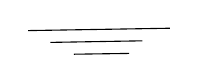
\begin{tikzpicture}[x=1cm,y=1cm]
\draw (0,0)--(1.8,.03);\draw (.28,-.15)--(1.45,-.13);\draw (.58,-.3)--(1.28,-.29);
\end{tikzpicture}}
\margin{\textcircled{c}}
Dans le cas \unsure{2)}, \inserted{$f$ et $g$ propres,} supposons que $S$ est discret,
\deleted{\unsure{bornés}}
\inserted{$F_\bullet,G_\bullet$ à \unsure{ch.} constructibles à tor.-dim finie,}
\deleted{\unsure{par dualité}}
\unsure{donc} on trouve
que $\operatorname{Hom}^{0}(\mathbb{R}f_*(F_\bullet),\mathbb{R}g_*(G_\bullet))$ et
$\operatorname{Hom}^{0}(\mathbb{R}g_*(G_\bullet),\mathbb{R}f_*(F_\bullet))$
\inserted{ou $\mathbb{R}\mathcal{H}om^\bullet(-,\cdot)$ et $\mathbb{R}\mathcal{H}om^\bullet(\cdot,-)$ \unsure{les}}
sont duaux l'un de l'autre; je dis que cette dualité est \uline{induite par un accouplement}
\diagram{\fbox{\begin{tikzcd}[ampersand replacement=\&,column sep=small]
\mathbb{R}\mathcal{H}om^\bullet(\deleted{\unsure{f^*}}\inserted{\operatorname{pr}_1^*}(F_\bullet),\operatorname{pr}_2^!(G_\bullet))\times \& \mathbb{R}\mathcal{H}om(\operatorname{pr}_2^*(G_\bullet),\operatorname{pr}_1^!(F_\bullet))\arrow[d]\\
\&K^\bullet_{X\times_S Y}=\deleted{\unsure{f}}\inserted{h}^!(A_S)
\end{tikzcd}}}
que l'on décrit ainsi (sans hyp. de propreté sur $f,g$ !) On a $Z=X\times_S Y$
\margin{147}
\scanpage{149}
\margin{148}
\mspage{9.}

\uline{Théorème 1.}- \uline{Soit} $X$ \uline{un préschéma. Considérons les sous-catégories pleines} $E$ \uline{de} $\overset{\inserted{\wedge}}{(\mathrm{Sch})_{/X}}$ \uline{qui sont des} $\underline{U}$-\uline{topos et dont les objets} $F$ \uline{satisfont aux axiomes}

(A) \uline{Pour tout} $X$-\uline{morphisme} $S\inserted{\xrightarrow{\varphi}}S'$ \uline{entre deux} $X$-\uline{préschémas affines dans le sens absolu tel que} $\inserted{\varphi}$ \uline{induise un homéomorphisme sur les espaces topologiques sous-jacentes, le morphisme évident}
\diagram{\begin{tikzcd}[ampersand replacement=\&]
F(S')\arrow[r,"F(\inserted{\varphi})"]\&F(S)
\end{tikzcd}}
\uline{est un isomorphisme,}

(B) \uline{Pour tout} $\underline{U}$-\uline{système projectif filtrant de préschémas} $\inserted{\{}S_{\inserted{\alpha}}\inserted{\}}$ \uline{où les} $S$ \uline{sont affines au-dessus d'un ouvert affine de} $X$ \uline{l'application évidente}
\diagram{\begin{tikzcd}[ampersand replacement=\&]
F(\varprojlim S_\alpha)\&\varinjlim F(S_\alpha)\arrow[l]
\end{tikzcd}}
\uline{est un isomorphisme,}

\uline{et restreignons-nous aux} $E$ \uline{qui de plus contiennent les objets représentables satisfaisant aux conditions} (A) \uline{et} (B). \uline{Parmi ces topos il y a un qui est} minimum \uline{i.e.\ est contenu dans tout autre} $E$. \uline{Ce topos} (évidemment unique ) \uline{est équivalent à} $\overset{\inserted{\sim}}{\operatorname{Ouv}(X)}$.

La démonstration du théorème 1 s'appuiera sur le lemme suivant qui sera démontré dans le \S\ 3.

\uline{Lemme 2.}- \uline{La condition nécessaire et suffisante pour qu'un objet} $Y/X\inserted{\in}(\mathrm{Sch})_{/X}\inserted{\hookrightarrow}(\mathrm{Sch})_{/X}$ \uline{satisfasse aux conditions} (A) \uline{et} (B) \uline{du théorème} 1, \uline{c'est que} $Y\inserted{\xrightarrow{f}}X$ \uline{soit un isomorphisme local.}
(Ceci signifie que chaque point de $Y$ admet un voisinage ouvert $U$ tel que $f\inserted{|}U:U\inserted{\longrightarrow}X$ soit une immersion ouverte \inserted{[}EGA I.4.5\inserted{]} )

\uline{Démonstration du théorème 1.}- Soit $\operatorname{Isloc}(X)$ la catégorie des isomorphismes locaux $Y/X$. Pour démontrer le théorème 1, il suffit de voir qu'il y a une équivalence de catégories
\diagram{\begin{tikzcd}[ampersand replacement=\&]
\overset{\inserted{\sim}}{\operatorname{Ouv}(X)}\arrow[r]\&\operatorname{Isloc}(X).
\end{tikzcd}}
\scanpage{150}
\[
\operatorname{pr}_2^!(G_\bullet)\longrightarrow\deleted{\unsure{\unsure{\underline{D}|D}_Z\unsure{\underline{D}|D}_Z}}\operatorname{pr}_2^!(\deleted{G_\bullet}\inserted{\unsure{\underline{D}|D}_Y(\unsure{\underline{D}|D}_Y(G_\bullet))})\xrightarrow{\sim}\unsure{\underline{D}|D}_Z\operatorname{pr}_2^*(\unsure{\underline{D}|D}_Y G)
\]
\inserted{iso si $\unsure{\underline{D}|D}_Y(G_\bullet)$ à ch.\ const.}

d'où
\diagram{\begin{tikzcd}[ampersand replacement=\&,column sep=small]
\mathbb{R}\mathcal{H}om(\operatorname{pr}_1^*(F_\bullet),\operatorname{pr}_2^!(G_\bullet))\arrow[r]\&\mathbb{R}\mathcal{H}om(\operatorname{pr}_1^*(F_\bullet),\unsure{\underline{D}|D}_Z\operatorname{pr}_2^*(\unsure{\underline{D}|D}_Y G))\arrow[d,phantom,"\simeq" description]\\
\&\unsure{\underline{D}|D}_Z(\operatorname{pr}_1^*(F_\bullet)\overset{\mathbb{L}}{\otimes}\operatorname{pr}_2^*(\unsure{\underline{D}|D}_Y G))
\end{tikzcd}}

Il suffit de décrire maintenant
\[
\unsure{\underline{D}|D}_Z(\operatorname{pr}_1^*(F_\bullet)\overset{\mathbb{L}}{\otimes}\operatorname{pr}_2^*(\unsure{\underline{D}|D}_Y G)))\unsure{\text{---}|\longrightarrow}\unsure{\underline{D}|D}_Z\mathbb{R}\mathcal{H}om^\bullet(\operatorname{pr}_2^*G,\operatorname{pr}_1^!(F_\bullet))
\]
\deleted{\unsure{i.e.}} ou encore un hom
\[
\mathbb{R}\mathcal{H}om^\bullet(\operatorname{pr}_2^*(G),\operatorname{pr}_1^!(F_\bullet))\longrightarrow\operatorname{pr}_1^*(F_\bullet)\overset{\mathbb{L}}{\otimes}\operatorname{pr}_2^*(\unsure{\underline{D}|D}_Y(G_\bullet)).
\]
Or le premier est \unsure{d'abord|d'après}, comme on a vu, \unsure{iso}
\[
\unsure{\underline{D}|D}_Z(\operatorname{pr}_2^*(G)\overset{\mathbb{L}}{\otimes}\operatorname{pr}_1^*(\unsure{\underline{D}|D}_X F_\bullet))
\]
donc tout revient à définir
\[
\unsure{\underline{D}|D}_Z(\operatorname{pr}_2^*(G)\overset{\mathbb{L}}{\otimes}\operatorname{pr}_1^*\unsure{\underline{D}|D}_X(F_\bullet))\longrightarrow\operatorname{pr}_1^*(F_\bullet)\overset{\mathbb{L}}{\otimes}\operatorname{pr}_2^*(\unsure{\underline{D}|D}_Y(G_\bullet)).
\]
\figure{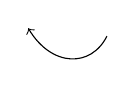
\begin{tikzpicture}[x=1cm,y=1cm]
\draw[->] (1,0)..controls(.8,-.4) and (.3,-.4)..(0,.1);
\end{tikzpicture}}
Pour ceci, nous allons définir un \uline{hom.\ en sens inverse}, et \uline{montrer que c'est un isomorphisme} (\unsure{cela en bonne dimension}!).

Or \deleted{\unsure{l'hom}}\inserted{donner} un \unsure{sens} inverse est équivalent à donner un accouplement
\margin{\textcircled{d}}
\[
\operatorname{pr}_1^*(F)\overset{\mathbb{L}}{\otimes}\operatorname{pr}_2^*\unsure{\underline{D}|D}_Y G_\bullet\overset{\mathbb{L}}{\otimes}\operatorname{pr}_2^*G\overset{\mathbb{L}}{\otimes}\operatorname{pr}_1^*\unsure{\underline{D}|D}_X(F_\bullet)\longrightarrow\deleted{\unsure{A}}K_Z^\bullet
\]
\margin{Plus explicite
\diagram{\begin{tikzcd}[ampersand replacement=\&,column sep=small]
\unsure{\mathbb{R}|\mathrm{R}}\mathcal{H}om^\bullet(\operatorname{pr}_1^*F,\operatorname{pr}_2^!G)\arrow[r]\&\unsure{\underline{D}|D}_Z\operatorname{pr}_1^*(F)\overset{\mathbb{L}}{\otimes}\operatorname{pr}_2^*(\unsure{\underline{D}|D}_Y G)\\
\unsure{\mathbb{R}|\mathrm{R}}\mathcal{H}om(\operatorname{pr}_1^*F,\operatorname{pr}_2^!G)\arrow[r]\&\unsure{\underline{D}|D}_Z\operatorname{pr}_2^*(G)\overset{\mathbb{L}}{\otimes}\operatorname{pr}_1^*(\unsure{\underline{D}|D}_X F)
\end{tikzcd}}
$\left.\vphantom{\begin{matrix}a\\b\end{matrix}}\right\}$ il faut accoupler les deuxièmes mb.\ \unsure{à valeurs} dans $K_Z^\bullet$.}
\margin{149}
\scanpage{151}
\margin{150}
\mspage{8.}

\uline{Résumé des propositions 2 et 3.}- \uline{Le foncteur}
$\overset{\inserted{\sim}}{\operatorname{Ouv}(X)}\inserted{\xrightarrow{i_X^*}}\overset{\inserted{\sim}}{(\mathrm{Sch})}_{/X}$
\uline{est pleinement fidèle et il admet un adjoint à droite qui commute aux} $\underline{U}$-$\varinjlim$ \uline{arbitraires. De plus} $i_X^{\inserted{*}}$ \uline{commute aux} $\varprojlim$ \uline{finies.}

Tout a été démontré sauf l'assertion ``$i_X^{\inserted{*}}$ pleinement fidèle''.
Mais ceci est clair, car
\[
\operatorname{Hom}_{\overset{\inserted{\sim}}{\operatorname{Ouv}(X)}}(F,G)=\operatorname{Hom}(F,i_{X\inserted{*}}i_X^{\inserted{*}}G)=
\]
\[
=\operatorname{Hom}(i_X^{\inserted{*}}F,i_X^{\inserted{*}}G).
\]

\uline{Remarque1}.Nos raisonnements dans ce paragraphe ne sont pas particuliers à la topologie de Zariski et nous rencontrerons plus tard un autre cas où ils s'appliquent.

\uline{Remarque 2.} Dans tout ce qui précède, les faisceaux,\inserted{et les} préfaisceaux ont leurs valeurs dans la catégorie des $\underline{U}$-ensembles. Le lecteur s'assurera (en utilisant la proposition 1 ) qu'il n'y a pas de difficulté due au fait que $(\mathrm{Sch})_{/X}$ n'appartient pas à $\underline{U}$. Le foncteur $i_X^\bullet$ existe, car $\operatorname{Ouv}(X)\in\underline{U}$. On pourrait aussi faire les raisonnements pour les $\underline{V}$-(pré)-faisceaux,où $\underline{V}$ est un univers tel que $(\mathrm{Sch})_{/X}\inserted{\in}\underline{V}$, et se restreindre aux $\underline{U}$-(pré)-faisceaux après.

\S\ 2. \uline{Caractérisation ``axiomatique'' de la topologie de Zariski.}

Dans le paragraphe précédent nous avons vu que l'étude de la cohomologie de Zariski d'un préschéma $X$ peut ou bien se faire sur un grand site $(\mathrm{Sch}/X,\mathrm{Zar})$ ou bien sur des petits sites que l'on peut choisir d'une manière bien adaptée au problème en question. Dans ``la pratique'' c'est surtout ce dernier point de vue qui est dominant. Mais du point de vue ``théorique'' c'est plus agréable d'étudier la topologie de Zariski sur $(\mathrm{Sch})_{/X}$, surtout quand on veut faire des comparaisons avec d'autres topologies sur des préschémas. C'est pour préparer l'étude de ces autres topologies que nous allons donner dans ce paragraphe une caractérisation axiomatique de la topologie de Zariski ou plus précisément du petit topos de Zariski.
\scanpage{152}

On a
\[
\operatorname{pr}_1^*(F)\otimes\operatorname{pr}_1^*(\unsure{\underline{D}|D}_X F))\unsure{\text{---}|\longrightarrow}\operatorname{pr}_1^*(K_X^\bullet)
\]
\[
\operatorname{pr}_2^*(G)\otimes\operatorname{pr}_{\unsure{2}}^*\unsure{\underline{D}|D}_Y G\unsure{\text{---}|\longrightarrow}\operatorname{pr}_2^*(K_Y)
\]
donc le premier mb de \textcircled{\scriptsize$\alpha$} s'en \unsure{va} dans
\[
\operatorname{pr}_1^*(K_X)\otimes\operatorname{pr}_2^*(K_Y)
\]
il faut l'envoyer \inserted{\unsure{canoniqt}} dans $K_Z^\bullet$. Ceci ne devrait pas offrir de difficulté --- p.ex.\ c'est trivial si $X$ ou $Y$ est lisse/$\unsure{k|S}$.
[en fait, \unsure{on trouve} que le produit tensor est $\sim K_Z^\bullet$].
\margin{ou si $X$ \unsure{et|ou} $Y$ sont lisses sur $\unsure{k}$, \unsure{sinon} \unsure{la|les} \unsure{vérification|vibrations} \unsure{des signes|des cônes} \unsure{inquiétante|inquiétants}\ldots!}
Cela définit bien l'accouplement voulu, d'où un \uline{hom.\ can.}
\margin{\textcircled{**}}
\[
\operatorname{pr}_1^*(F_\bullet)\otimes\operatorname{pr}_2^*(\unsure{\underline{D}|D}_Y(G_\bullet))\longrightarrow\unsure{\underline{D}|D}_Z(\operatorname{pr}_2^*G\otimes\operatorname{pr}_1^*\unsure{\underline{D}|D}_X(F))
\]

\uline{Lemme fondamental de Verdier}: \uline{Cet homomorphisme est un isomorphisme}

\deleted{\uline{Dém.}\ On est ramené comme d'habitude au cas où \inserted{$X,Y$ affines,} $F_\bullet,G_\bullet$ sont de la forme $i_!(A_U)$, $j_!(A_V)$, où $i:U\longrightarrow X$, $j:V\longrightarrow X$ étales, avec $U,V$ affines.}
\margin{151}
\scanpage{153}
\margin{152}
\mspage{7.}

Pour compléter l'étude des relations entre le petit site $\operatorname{Ouv}(X)$ et le site $(\mathrm{Sch}/X,\mathrm{Zar})$, il reste à démontrer que chaque faisceau sur $\operatorname{Ouv}(X)$ est l'image par $i_{X\inserted{*}}$ d'un faisceau de Zariski sur $(\mathrm{Sch})_{/X}$. Ceci montrera en particulier, en vertu de l'isomorphisme (2), que la cohomologie de $\operatorname{Ouv}(X)$ pourra \inserted{ê}tre calculé dans $(\mathrm{Sch}/X,\mathrm{Zar})$. Plus précisément, nous avons le résultat suivant:

\uline{Proposition} 3.- \uline{Pour chaque} $F\inserted{\in}\overset{\inserted{\sim}}{\operatorname{Ouv}(X)}$, \uline{le morphisme naturel}
\[
F\inserted{\longrightarrow}i_{X\inserted{*}}i_X^{\inserted{*}}F
\]
\uline{est un isomorphisme.}

\uline{Démonstration:} Il suffit de démontrer que
\[
F(U)\inserted{\longrightarrow}(i_{X\bullet}ii_X^{\inserted{*}}F)(U)=(i_X^{\inserted{*}}F)(i_X(U))
\]
est un isomorphisme pour tout $U\inserted{\in}\operatorname{Ouv}(X)$. Il suffit m\inserted{ê}me de démontrer que
\[
F(U)\inserted{\longrightarrow}(i_X^\bullet F)(i_X(U))
\]
est un isomorphisme pour tout $U$. Rappelons que
\[
(i_X^\bullet F)(Y)=\varinjlim_{I_{i_X}^{Y\,o}}F(V)
\]
où $I_{i_X}^{Y}$ est la catégorie des paires $\inserted{\{}V,Y\inserted{\xrightarrow{\varphi}}i_X(V)\inserted{\}}$ $(Y\inserted{\in}(\mathrm{Sch})_{/X})$ avec, comme morphismes entre deux telles paires, les $V\inserted{\xrightarrow{j}}V'$ tels que le diagramme
\diagram{\begin{tikzcd}[ampersand replacement=\&]
\&Y\arrow[dl,"\inserted{\varphi}"']\arrow[dr,"\inserted{\varphi'}"]\&\\
i_X(V)\arrow[rr,"i_X(j)"]\&\&i_X(V')
\end{tikzcd}}
soit \uline{commutatif} (dans $(\mathrm{Sch})_{/X}$ ). Cette catégorie est pseudo-filtrante à gauche et connexe, car $i_X$ commute aux limites projectives finies. Dans le cas qui nous intéresse, $Y=i_X(U)$, il est facile de voir qu'il existe \inserted{en outre} un objet final dans la catégorie $I_{i_X}^{Y\,o}$, à savoir $\inserted{\{}U,i_X(U)\inserted{\xrightarrow{\mathrm{Id}}}i_X(U)\inserted{\}}$, d'où le résultat.
\scanpage{154}

L'existence d'un hom can (en fait un \uline{isom.})
\[
\text{(1)}\qquad \unsure{R|K}_X^\bullet\overset{\mathbb{L}}{\boxtimes}\unsure{R|K}_Y^\bullet\xrightarrow{\sim}\unsure{R|K}_{X\times Y}^\bullet
\]
et \unsure{du fait} que l'accouplement de Verdier donne un isomorphisme
\[
\text{(2)}\qquad\deleted{\unsure{\operatorname{pr}}}F_\bullet\overset{\mathbb{L}}{\boxtimes}\unsure{\underline{D}|D}_Y G_\bullet\xrightarrow{\sim}\unsure{\underline{D}|D}_Z(\deleted{\unsure{F}}\unsure{\underline{D}|D}_X F_\bullet\overset{\mathbb{L}}{\boxtimes}G_\bullet)
\]
résulte de la formule générale (appliquée deux fois)
\margin{``\uline{Künneth local}''}
\[
\boxed{\mathbb{R}\mathcal{H}om(F_\bullet\overset{\mathbb{L}}{\boxtimes}G_\bullet,P_\bullet\overset{\mathbb{L}}{\boxtimes}Q_\bullet)\xleftarrow{\sim}\mathbb{R}\mathcal{H}om(F_\bullet,P_\bullet)\overset{\mathbb{L}}{\boxtimes}\mathbb{R}\mathcal{H}om(G_\bullet,Q_\bullet)}
\]
\inserted{$\mathbb{R}^!(f\times g)^{\unsure{!}}(P_\bullet\overset{\mathbb{L}}{\boxtimes}Q_\bullet)\simeq\mathbb{R}^!f(P_\bullet)\overset{\mathbb{L}}{\boxtimes}\mathbb{R}^!g(Q_\bullet)$}
valable si $F_\bullet,G_\bullet$ sont de tor-dim finie à ch.\ constructible, et $P_\bullet,Q_\bullet$ \deleted{à tor dim finie} \inserted{$\in\operatorname{Ob}D^{\unsure{-|+}}\deleted{\unsure{c}}$}
($A=\mathbb{Z}/n\mathbb{Z}$, $n$ premier à car $k$),
formule valable si sur les schémas \unsure{ambiants} $U,V$, \inserted{et ceux \unsure{qui sont propres} sur eux,} la résolution des singularités à la Hironaka est possible (O.K.\ en car.\ 0, et en car.\ $p$ quelcon.\ si $U,V$ de dim $\leq2$).
NB.\ Dans le cas (1), on se ramène à prendre pour $U,V$ des schémas lisses qui contiennent $X,Y$ --- \unsure{ce qui est évident dès}
\margin{153}
\scanpage{155}
\margin{154}
\uline{Réédition d'E. V. T.\ ,chap.\ II} \mspage{(14)}
\margin{Tribu n\textsuperscript{o} 63}

Remplacer les l.\ 6-11 du bas (d'ailleurs canulées si on n'a pas rectifié l.\ 11) par une récurrence sur $n$: $x=x_1$ ou $x$ barycentre de $x_2,\ldots,x_n$.

P.\ 115, l.\ 4, une référence pour $B(\mathbb{N})$.

Remplacer l'exemple 3 par: soit $u:C\longrightarrow C'$ où $C$ et $C'$ sont convexes et $u$ affine; soient $x$ un point extrémal de $C'$, $y$ un point extrémal de $u^{-1}(x)$; alors $y$ est extrémal dans $C$.

l.\ 6 du bas: compact non vide.

P.\ 116, l.\ 6, (i), (ii) et (iii) sont également triviaux.

P.\ 117, l.\ 1: Puisque $E$ est elc séparé, il suffit de voir \ldots

Vider les cor.\ 1, 2, 3.

P.\ 118, démonstration du th.\ 1: D'après la prop.\ 1, toute fonction affine continue $\geq0$ sur $B$ est $\geq0$ sur $A$. Donc $B=A$ (s'assurer qu'on a bien mis au \S\ de la séparation des convexes exactement ce qu'il faut).

P.\ 118 et 119, échanger la prop.\ 2 et son corollaire. Démonstration du corollaire: Pour tout demi-espace ouvert $D$ contenant $x$, soit $L_D=(E-D)\cap A$ qui est convexe compact. $A-\{x\}$ est convexe, donc $\Gamma(L_D\cup L_{D'})$ ne contient pas $x$, et est compact. Donc les $L_D$ sont filtrant décroissants. Les $L\cap\bar D$ ont pour intersection $x$, et forment un système fondamental de voisinages de $x$. Démonstration de la prop.\ 2: Si $K$ laisse échapper un point extrémal $x$, il laisse échapper une tranche voisinage de $x$, donc $\overline{\Gamma(K)}\neq A$.

Exercice: dans le cor., remplacer $x$ par un chapeau.

P.\ 120, la conjecture de la l.\ 9 est fausse. Voici une contre-exemple (exercice: deviner l'auteur): soit $B$ la boule unité d'un Hilbert faible $H$; $x\in$ sphère unité; il n'y a qu'un hyperplan d'appui; celui-ci disparaît si on affaiblit encore un peu la topologie faible (en utilisant un sous-espace partout dense bien choisi de $H$ ).

l.\ 10 du bas: un cône convexe.

l.\ 8 du bas, ajouter: Si $x\in D$ et $x=y+y'$ ($y,y'\in C$) alors $y,y'\in D$, et ceci caractérise les génératrices extrémales. (La Remarque 1, p.\ 121, devra alors être abrégée).

l.\ 5 du bas: $H$ un hyperplan contenant $x_o$.

P.\ 121, après la déf.\ 3, un exemple: * soient $X$ localement compact, $f$ une fonction
\scanpage{156}

dimensions \unsure{prohibitives}, qui peuvent empêcher d'appliquer la résolution. Il semble préférable alors \deleted{\unsure{de}} (si $X,Y$ ne sont pas encore lisses) de \deleted{\unsure{au}} \unsure{l'utiliser|d'utiliser} localement des homomorphismes \inserted{finis} $X\longrightarrow X'$, $Y\unsure{\text{---}|\longrightarrow}Y'$ avec $X'$ ($Y'$) lisse de dim ($\leq\dim X$) ($\leq\dim Y$) et de noter que grâce à l'interprétation de $\varphi^{\unsure{!|'}},\psi^{\unsure{!|'}}$ par des morphismes \uline{finis} $\varphi,\psi$, on a bien
\[
(\varphi\times\psi)^!\deleted{\unsure{\varphi^!}}(P_\bullet\boxtimes Q_\bullet)\simeq\varphi^!(P_\bullet)\boxtimes\psi^!(Q_\bullet)
\]
ce qui revient à
\[
\mathbb{R}\mathcal{H}om(F_\bullet\boxtimes G_\bullet,P_\bullet\boxtimes Q_\bullet)\simeq\mathbb{R}\mathcal{H}om(F_\bullet,P_\bullet)\overset{\mathbb{L}}{\boxtimes}\mathbb{R}\mathcal{H}om(G_\bullet,Q_\bullet)
\]
avec $F_\bullet=\varphi_*(A_X)$, $G_\bullet=\psi_*(A_Y)$ ----
\margin{\diagram{\begin{tikzcd}[ampersand replacement=\&]
X\arrow[d,"\varphi"]\&Y\arrow[d,"\psi"]\\
X'\&Y'
\end{tikzcd}}}
\margin{155}
\scanpage{157}
\margin{156}
\uline{Réédition des E. V. T., chap. II} \mspage{(13)}
\margin{Tribu n\textsuperscript{o} 63}

complète de $F$ ne contenant aucune droite affine. Alors l'application $(x,y)\mapsto x+y$ de $C\times C$ dans $F$ est propre.

Démonstration. On complète $F$ qui devient un $\mathbb{R}^{I}$, avec $C\subset\mathbb{R}^{I}_{+}$. En utilisant les produits d'applications propres (Top. gén. I, § 10, n\textsuperscript{o} 2, cor. 3 du th. 1) et les restrictions (loc. cit., n\textsuperscript{o} 1, cor. 1 de la prop. 5), on est ramené au cas où $F=\mathbb{R}$. Alors le critère de propreté par les compacts suffit pour s'en tirer.

Corollaire 3. Supposer seulement que $F$ est faible séparé et que $C$ est complet. Dans (ii), $A$, $B$, $C$ doivent être complets, mais seul $C$ doit être convexe.

P. 102, la prop. 11 a été remontée, sauf la dernière phrase qui est fausse (elle impliquerait que $\mathcal{M}(\unsure{x|X})$ vague serait métrisable).

Le n\textsuperscript{o} 9 est entièrement vidé (il restera au chap. IV), et le cor. 3 de la p. 110 est vidé définitivement.

Le n\textsuperscript{o} 10, très réduit, ira en § 7, n\textsuperscript{o} 2.

Le lemme 2 devient une proposition.

P. 110, l. 6 du bas, vider égal à $\bigcup\lambda K$ ; vider dans $E$.

l. 5 du bas, vider faiblement.

l. 1 du bas, l'enveloppe convexe $A$.

P. 111, à partir de la l. 7, pas de $B_n$. Il est clair que $C_n$ est compact (image continue d'un compact), $C$ est réunion des $C_n$ ; il existe un voisinage fermé $V$ de $0$ dans $E$ tel que, pour tout $x\in E$, $(x+V)\cap C\subset C_n$ pour $n$ assez grand. Donc $C$ est fermé et localement compact, et tout filtre de Cauchy ``est'' sur l'un des $C_n$.

l. 3 du bas : définir les semelles d'un cône quelconque dans un espace vectoriel

P. 112, l. 1, supposer $E$ séparé.

Depuis la l. 3 (et réciproquement) jusqu'à la p. 113, l. 5 du bas, tout est vidé sauf la prop. 17 (i) qui devient Exemple 1, et l'Exemple 1 qui devient Exemple 2.
Les l. 1-5 du bas de la p. 113 deviennent Exemple 3.

P. 114, l. 1-5 vidées.

l. 11, ajouter $y\ne z$.

l. 12, ajouter que ça équivaut à : $A-\{x\}$ convexe.

l. 14, remplacer identique par égal.
\scanpage{158}
\margin{\textcircled{\unsure{d|e}}}
\deleted{Cela \unsure{par}}

On a donc trouvé un accouplement (\unsure{commutant|donnant} \unsure{à|:} la \unsure{permutation|multiplication} à un \unsure{signe})
\diagram{\begin{tikzcd}[ampersand replacement=\&,column sep=small,row sep=large]
\mathbb{R}\mathcal{H}om(\mathrm{pr}_1^*(F_\bullet),\mathrm{pr}_2^!(G_\bullet))\times\arrow[d,no head,bend left=25]
\&\mathbb{R}\mathcal{H}om(\mathrm{pr}_2^*(G_\bullet),\mathrm{pr}_1^!(F_\bullet))\arrow[r]\arrow[d,no head,bend left=35]
\&K_{X\times_S Y}^{\bullet}\\
\deleted{\text{D'où, pour }\xi^0\in\mathbb{R}^0\Gamma_{X\times_S Y}(\quad)}
\&\deleted{\text{et }\eta^0\in\mathbb{R}^0\Gamma_{X\times_S Y}(\quad)}\&
\end{tikzcd}}
\deleted{un élément $\unsure{\xi^0\cup\eta^0}$}
\deleted{$\xi^0\cup\eta^0\in\mathbb{R}^0\Gamma_{X\times_S Y}(K_{X\times_S Y}^{\bullet})$}

Appliquant $\mathbb{R}\Gamma_{X\times_S Y}$, on trouve un accouplement
\diagram{\begin{tikzcd}[ampersand replacement=\&,column sep=small]
\mathbb{R}\operatorname{Hom}^{\bullet}(\mathrm{pr}_1^*(F),\mathrm{pr}_2^!(G))\times \arrow[d,phantom,"\simeq" description]
\& \mathbb{R}\operatorname{Hom}^{\bullet}(\mathrm{pr}_2^*(G),\mathrm{pr}_1^!(F)) \arrow[r] \arrow[d,phantom,"\simeq" description]
\& \mathbb{R}\Gamma_{X\times_S Y}K_{X\times_S Y}^{\bullet}\arrow[d]\\
\mathbb{R}\operatorname{Hom}^{\bullet}(\unsure{\mathbb{R}f_*}(F),\unsure{\mathbb{R}g_*}(G))\times
\& \mathbb{R}\operatorname{Hom}^{\bullet}(\unsure{\mathbb{R}g_*}(G),\unsure{\mathbb{R}f_*}(F))\arrow[r]
\& \deleted{\unsure{\mathbb{R}}}A_S
\end{tikzcd}}
qui ne doit être autre que l'accouplement déjà connu \unsure{relatif} ; $P_\bullet\simeq\unsure{\mathrm{pr}_{1*}|\mathbb{R}f_*}(F_\bullet)$ et $Q_\bullet\simeq\unsure{\mathrm{pr}_{2*}|\mathbb{R}g_*}(G_\bullet)$.

En particulier, si
\[
\xi^0\in\mathbb{R}^0\operatorname{Hom}^{\bullet}(\mathrm{pr}_1^*(\unsure{P|F}),\mathrm{pr}_2^!(\unsure{Q|G}))
=\mathbb{R}^0\Gamma_{X\times_S Y}\,\mathbb{R}\mathcal{H}om(\mathrm{pr}_1^*(F),\mathrm{pr}_2^!(G_\bullet))
\]
\[
\eta^0\in\mathbb{R}^0\operatorname{Hom}^{\bullet}(\mathrm{pr}_2^*(\unsure{Q|G}),\mathrm{pr}_1^!(F))
=\mathbb{R}^0\Gamma_{X\times_S Y}\,\mathbb{R}\mathcal{H}om(\mathrm{pr}_1^*(F),\mathrm{pr}_2^!(G_\bullet))
\]
alors
\[
\xi^0\cup\eta^0\in\mathbb{R}^0\Gamma_{X\times_S Y}(K_{X\times_S Y}^{\bullet})\xrightarrow{\operatorname{Tr}_h} A.
\]
et on aura
\[
\boxed{\operatorname{Tr}(\xi^0\cup\eta^0)=\langle\xi^0,\eta^0\rangle}
\qquad
\left(=\sum_i\operatorname{Tr}(\xi^0)^{(i)}(\eta^0)^{(\unsure{-i|i})}\unsure{(-1)^i}\right)
\]
\figure{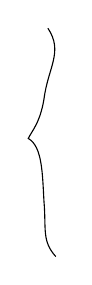
\begin{tikzpicture}[x=1cm,y=1cm]
\draw (.25,1.4)..controls(.45,1.1) and (.25,.9)..(.2,.5)..controls(.15,.2) and (.05,.1)..(0,0)..controls(.18,-.1) and (.18,-.45)..(.2,-.8)..controls(.23,-1.15) and (.17,-1.3)..(.35,-1.5);
\end{tikzpicture}}
\margin{si on représente $\unsure{f_*}(P),\unsure{g_*}(Q)$ par des complexes plats de type fini en chaque degré !).}
\margin{157}
\scanpage{159}
\mspage{4.}
\margin{158}
\uline{les} $j_\alpha$ \uline{sont des immersions ouvertes dont les images recouvrent} $Z$ (ceci est bien une prétopologie). \uline{Cette topologie s'appelle la} topologie de Zariski \uline{sur} $(\mathrm{Sch})_{/X}$ \uline{et le site correspondant sera noté} $(\mathrm{Sch}/X,\mathrm{Zar})$. \uline{Toute notion associée à ce site sera qualifiée ``de Zariski''} (faisceaux, cribles couvrants etc. )

\uline{Remarque.} - Si $Z\longrightarrow X$ est un morphisme dans $(\mathrm{Sch})$, nous avons $(\mathrm{Sch})_{/Z}=(\mathrm{Sch})_{/X}\big/ Z/X$ et la topologie sur $(\mathrm{Sch})_{/X}$ que nous venons de construire induit bien la topologie analogue sur $(\mathrm{Sch})_{/Z}$. En particulier, on voit en prenant $X=\operatorname{Spec}(\mathbb{Z})$ que le site $(\mathrm{Sch},\mathrm{Zar})$ détermine les sites $(\mathrm{Sch}/Y,\mathrm{Zar})$, $Y\in(\mathrm{Sch})$.

\uline{Démonstration de la proposition 1.}- Il suffit de montrer que les deux conditions suivantes sur $F\in\widehat{(\mathrm{Sch})_{/X}}$ sont équivalentes:

(i) Pour tout $Z/X\in(\mathrm{Sch})_{/X}$, $i_{Z\bullet}(F)\in\widetilde{\mathrm{Ouv}(Z)}$

(ii) Pour chaque $Z/X$ et pour chaque famille couvrante $\{Z_\alpha\longrightarrow Z\}$ de $Z/X$ la suite
\diagram{\begin{tikzcd}[ampersand replacement=\&]
(1)\quad F(Z)\arrow[r]\&\displaystyle\prod_\alpha F(Z_\alpha)\arrow[r,shift left]\arrow[r,shift right]\&\displaystyle\prod_{\alpha,\beta}F(Z_\alpha\mathop{\prod}\limits_Z Z_\beta)
\end{tikzcd}}
est exacte.

D'abord il est clair que (ii) $\Longrightarrow$ (i). Car si $U$ est un ouvert de l'espace topologique sous-jacent à $X$ et $\{U_\alpha\}$ un recouvrement de $U$ par des ouverts, il est clair que les $(\mathrm{Sch})_{/X}$-morphismes $i_Z(U_\alpha)\longrightarrow i_Z(U)$ sont des immersions ouvertes dont les images recouvrent $i_Z(U)$. De plus, nous avons un isomorphisme évident entre $i_Z(U_\alpha)\mathop{\prod}\limits_{i_Z(U)} i_Z(U_\beta)$ et $i_Z(U_\alpha\cap U_\beta)$. Comme $(i_{Z\bullet}F)(U)=F(i_Z(U))$, un $F$ qui satisfait à (ii) vérifie bien (i).

Soit d'autre part $F$ un préfaisceau avec la propriété (i) et démontrons (ii). Comme les $Z_\alpha\xrightarrow{j_\alpha}Z$ sont des immersions ouvertes on peut les factoriser : $Z_\alpha\longrightarrow j_\alpha(Z_\alpha)\hookrightarrow Z$ où le premier morphisme est un isomorphisme de préschémas et où $j_\alpha(Z_\alpha)$ est le préschéma induit sur un ouvert de $Z$. Il est facile de voir que la suite (1) est exacte si et seulement si la suite analogue pour la famille $\{j_\alpha(Z_\alpha)\longrightarrow Z\}$ l'est. Or ceci est
\scanpage{160}
En particulier, si $X=Y$, $F=G$, prenant $\eta^0=\deleted{\unsure{\alpha}}\delta_{X,F}$ on trouve
\[
\boxed{\operatorname{Tr}(\xi^0\cup\delta_{X,F}^{0})=\sum\unsure{(-1)^i}\operatorname{Tr}[\xi^0]^i}
\]
C'est la \uline{formule de Lefschetz-Verdier}.

\margin{\textcircled{e}\quad 2}
\deleted{\unsure{\S}}
Considérons un morphisme
\[
u:T\longrightarrow X\times_S Y
\]
\unsure{défini} donc par deux morphismes
\[
u_1:T\longrightarrow X,\quad u_2:T\longrightarrow Y.
\]
On a alors un morphisme évident
\[
\mathbb{R}u_*\bigl(\mathbb{R}\mathcal{H}om(u_1^*(F_\bullet),u_2^!(G_\bullet))\bigr)
\longrightarrow\mathbb{R}\mathcal{H}om(\mathrm{pr}_1^*(F),\mathrm{pr}_2^!(G_\bullet))
\]
Car $u_i=\mathrm{pr}_i u$, donc le premier est un
\diagram{\begin{tikzcd}[ampersand replacement=\&,column sep=large,row sep=large]
\mathbb{R}u_*\bigl(\mathbb{R}\mathcal{H}om(\deleted{\unsure{\mathrm{pr}}}u^*\mathrm{pr}_1^*(F),u^!(\mathrm{pr}_2^!(G_\bullet)))\bigr)\arrow[r,"\sim"]\arrow[d,phantom,"\simeq" description]
\&\mathbb{R}\mathcal{H}om(\mathrm{pr}_1^*(F),u_*u^!(\mathrm{pr}_2^!(G)))\arrow[d,"\varepsilon"]\\
\mathbb{R}\mathcal{H}om(u_*u^*(\mathrm{pr}_1^*(F)),\mathrm{pr}_2^!(G_\bullet))\arrow[r]
\&\mathbb{R}\mathcal{H}om(\mathrm{pr}_1^*(F),\mathrm{pr}_2^!(G))
\end{tikzcd}}

\deleted{Donc} tout élément de \deleted{$\unsure{\operatorname{Corr}^{0}(X,F,)}$}
\[
\alpha^0\in\mathbb{R}\operatorname{Hom}^{0}(u_1^*(F),u_2^!(G))
=\mathbb{R}^{0}\Gamma_T\bigl(\mathbb{R}\mathcal{H}om(u_1^*(F),u_2^!(G_\bullet))\bigr)
\]
définit un \unsure{élément}
\[
\overline{\alpha^0}\in\operatorname{Corr}(X,F;Y,G)
\]
De même, un élément $\beta^0$ de $\mathbb{R}\operatorname{Hom}^{0}(u_1^*(F),u_2^!(G))$ définit un \unsure{élmt} $\overline{\beta}\in\operatorname{Corr}(Y,G;X,F)$.
\margin{159}
\scanpage{161}
\mspage{3.}
\margin{160}
Les sites annelés $\mathrm{Ouv}(X)$ et $\mathrm{Ouv}(Y)$ sont donc isomorphes. Ils ont donc la m\inserted{ê}me cohomologie et, de plus, leurs faisceaux (quasi-) cohérents, localement libres etc. se correspondent, d'où la relation avec la théorie classique. Pour plus de détails voir \inserted{[}EGA IV , § 10\inserted{]} déjà cité.

Nous rencontrons déjà ici un fait qui va \inserted{ê}tre illustré plus abondamment dans ce qui suit : ``dans la pratique'' un site n'est pas donné d'une façon intrinsèque. Ici les sites $\mathrm{Ouv}(X)$ et $\mathrm{Ouv}(Y)$ sont cependant équivalentes (et m\inserted{ê}me isomorphes ). On verra que la catégorie des faisceaux associée à un site (i.e. le topos associé ) est beaucoup plus intrinsèque. Choisir un site particulier admettant un topos donné comme topos associé est une opération du m\inserted{ê}me genre que de choisir un système de générateurs d'un espace vectoriel, et il est naturel de chercher un tel site qui est aussi ``petit'' que possible.

On peut cependant introduire à l'aide des sites $\mathrm{Ouv}(Z)$ ($Z/X\in(\mathrm{Sch})_{/X}$) une topologie bien déterminée sur $(\mathrm{Sch})_{/X}$ de la manière suivante:

L'application qui a chaque ouvert de Zariski d'un préschéma $Z$ associe le préschéma induit sur cet ouvert définit un foncteur
\[
\mathrm{Ouv}(Z)\xrightarrow{i_Z}(\mathrm{Sch})_{/Z}
\]
d'où un foncteur sur les catégories des préfaisceaux
\[
\widehat{\mathrm{Ouv}(Z)}\xleftarrow{i_{Z\bullet}}\widehat{(\mathrm{Sch})_{/Z}}
\]

\uline{Proposition et définition 1.}-\uline{La sous-catégorie} (strictement) \uline{pleine de} $\widehat{(\mathrm{Sch})_{/X}}$ \uline{formée des préfaisceaux} $F$ \uline{tels que} $i_{Z\bullet}(F)\in\widetilde{\mathrm{Ouv}(Z)}$ \uline{pour tout} $Z/X\in(\mathrm{Sch})_{/X}$ \uline{est une catégorie de} $\underline{U}$-\uline{faisceaux sur} $(\mathrm{Sch})_{/X}$. \deleted{\illegible{5}} \uline{La topologie correspondante sur} $(\mathrm{Sch})_{/X}$ \uline{peut \inserted{ê}tre engendrée par la prétopologie où une famille} $\{Z_\alpha\xrightarrow{j_\alpha}Z\}_{\alpha\in I}$ \uline{de morphismes de} $(\mathrm{Sch})_{/X}$ \uline{est une famille couvrante si et seulement si}
\scanpage{162}
\margin{\diagram{\begin{tikzcd}[ampersand replacement=\&,column sep=small,row sep=small]
\&\unsure{\overline{T}|T}\times_Z T'\arrow[dl]\arrow[dr]\&\\
T\arrow[dr]\&\&T'\arrow[dl]\\
\&X\times_S Y=Z\&
\end{tikzcd}}\quad\unsure{f}\quad *}
À vrai dire, \deleted{\unsure{et}} si $\overline{T}$ est l'image de $T$ dans $Z=X\times_S Y$, on voit que $\overline{\alpha^0}$ ``est'' dans \deleted{l'image}
\[
\mathbb{R}^0\Gamma_{\overline{T}}(\mathbb{R}\mathcal{H}om(\mathrm{pr}_1^*(F),\mathrm{pr}_2^!(G_\bullet))
=\mathbb{R}^0\Gamma_{X\times_S Y}(\mathbb{R}^0\underline{\Gamma}_{\overline{T}}\mathbb{R}\mathcal{H}om(\,,))
\]
et de même $\overline{\beta^0}$ ``est \deleted{\unsure{dans l'image}}\inserted{même}'' dans
\[
\mathbb{R}^0\Gamma_{\overline{T}'}(\mathbb{R}\mathcal{H}om(\mathrm{pr}_2^*(G),\mathrm{pr}_1^!(F))
=\mathbb{R}^0\Gamma_{X\times_S Y}(\mathbb{R}^0\underline{\Gamma}_{\overline{T}'},\mathbb{R}\mathcal{H}om
\]
Ainsi, on peut définir un cup-produit
\[
\overline{\alpha^0}\cup\overline{\beta^0}\in
\mathbb{R}^0\Gamma_{\overline{T}\cap\overline{T}'}K_{\unsure{\infty}X\times_S Y}^{\bullet}
\simeq\mathbb{R}^0\Gamma_{\overline{T}\cap\overline{T}'}K_{\overline{T}\times_S\overline{T}'}^{\bullet}
\]
Ceci permet donc de définir, si
\[
\overline{T}\cap\overline{T}'=\bigcup_\alpha S_\alpha,
\]
\deleted{\unsure{réunion}} les $S_\alpha$ ouverts deux à deux disjoints (en nb fini) de définir des composantes canoniques
\[
(\overline{\alpha^0}\cup\overline{\beta^0})_\alpha:
\deleted{\unsure{\in H^0(S_\alpha,K_{S_\alpha}^{\bullet})}}
\]
et des $\deleted{\unsure{\operatorname{Tr}_{S_\alpha}}}\langle\xi^0,\eta^0\rangle_{S_\alpha}$ telles que
\[
\langle\xi^0,\eta^0\rangle=\sum_\alpha\langle\xi^0,\eta^0\rangle_{S_\alpha}
\]
\uline{Exemple} Supposons $\overline{T}\cap\overline{T}'=\varnothing$. Alors le nb de Lefschetz est nul.
\margin{161}
\scanpage{163}
\margin{162}
\begin{center}
INSTITUT DES HAUTES ETUDES SCIENTIFIQUES

Séminaire sur la topologie étale 1963-1964

Exposé VII

\uline{Topologies sur la catégories des préschémas.- Caractérisation}

\uline{``axiomatique'' de la topologie étale.}

par

JAN-ERIK ROOS
\end{center}

Nous allons maintenant introduire et étudier certaines topologies utiles sur $(\mathrm{Sch})=$ la catégorie des préschémas dans un univers $\underline{U}$ fixé dès maintenant (*). Nous utiliserons librement la terminologie et les résultats des exposés précédents. Souvent nous désignerons de la m\inserted{ê}me lettre un préschéma et son espace topologique sous-jacent. La m\inserted{ê}me remarque vaut pour un site et sa catégorie sous-jacente, une catégorie et l'ensemble de ses objets etc.

§ 1. \uline{La topologie de Zariski sur} $(\mathrm{Sch})$. \uline{Relations avec la géométri\inserted{e} algébrique ``classique''.}

Soit $X\in\underline{U}$ un préschéma. L'espace topologique sous-jacent à $X$ définit un site $\mathrm{Ouv}(X)\inserted{\in\underline{U}}$ (le site ``de Zariski'' de $X$ ). C'est la cohomologie de ce site (pour certains faisceaux et certains $X$) qui a été étudiée en détail dans la géométrie al\inserted{g}ébrique ``classique''. A vrai dire ce n'est pas exactement ce site qu'on a considéré au début, mais seulement le site analogue défini sur le sous-espace $X_o$ de $X$ formé des points \uline{fermés} de $X$. Précisons ceci: On dit qu'un préschéma $X$ est un \uline{préschéma de Jacobson} si le foncteur $\mathrm{Ouv}(X)\xrightarrow{\cap}\mathrm{Ouv}(X_o)$ défini par $U\rightsquigarrow U\cap X_o$ induit une équivalence des catégories des faisceaux d'ensembles (ou une équivalence des catégories des faisceaux abéliens, c'est la m\inserted{ê}me chose $\ldots$ ) sur ces deux sites.

\margin{\figure{\begin{tikzpicture}\draw (0,0)--(5.5,0);\end{tikzpicture}} (*) Nous dirons qu'un préschéma $(X,O_X)$ appartient à l'univers $\underline{U}$ si $X\in\underline{U}$ et si de plus $O_X$ est un faisceau de $\underline{U}$-ensembles.}
\scanpage{164}
\begin{flushright}
Compléments\\
dualité
\end{flushright}
\figure{\begin{tikzpicture}\draw (0,0) .. controls (.2,.15) and (.55,.20) .. (.8,.40);\end{tikzpicture}}
\margin{163}
\scanpage{165}
\margin{$\operatorname{cdim\,inj}F\leq 2\dim\unsure{\operatorname{Supp}F|X_{\operatorname{Supp}F}}+\sup_{x\in X}\dim\operatorname{inj}F_{\bar{x}}$}
\begin{center}
INSTITUT\\
DES HAUTES ÉTUDES SCIENTIFIQUES
\end{center}
\uline{Applications} --- \uline{possibles}

\textcircled{1} Majoration de la cdim. inj. via la dim inj. des fibres

Dim. ch. \unsure{stricte|stricts} d'un préschéma (en particulier d'un pr. Alg.)

(Consulter notes de Verdier)
\margin{$\operatorname{c-dim\,inj}(F)\leq\displaystyle\sup_{x\in X,\,F_{\bar{x}}\ne0}\left[2\dim O_{X,\bar{x}}+\dim\operatorname{inj}F_{\bar{x}}\right]$}

\figure{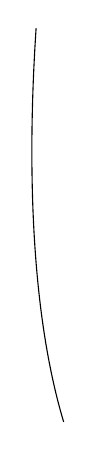
\begin{tikzpicture}[x=1cm,y=1cm]
\draw (0,0)..controls(-.1,-1.5) and (-.1,-3.5)..(.35,-5.0);
\end{tikzpicture}}
\textcircled{2} Cas d'un Anneau $A$ de torsion \uline{loc.} \uline{ct} premier aux car. résiduelles, et $R_X$ complexe de faisceaux de $A_X$-modules \unsure{\{}loc. cts, dualisant fibre par fibre (sur $X$ régulier ---)

\uline{NB} On peut globaliser, et considérer des schémas relatifs sur $(X_{\text{ét}},(\mathbb{Z}/n\mathbb{Z})_X)$ ----.

\textcircled{3} \deleted{Applications aux ths. de Lefschetz cohomologiques locaux et globaux [\unsure{Pourrait|Pourrais} donner un article séparé ....]}
\margin{164}
\scanpage{166}
\uline{Sujets de recherches}

a) $\bigwedge^i$ dans catégories dérivées, $\lambda$-anneaux et structures annexes

\diagram{$\left\{\begin{array}{ll}
\text{b)}&\text{Dualité analytique}\\[1em]
\text{c)}&\text{Descente cohomologique et}\\
&\text{applications (finitude}\\
&\text{analytique et algébrique ....)}
\end{array}\right.$}

\diagram{$\left\{\begin{array}{ll}
\text{d)}&\text{Künneth pour complexes}\\
&\text{quasi-cohérents}\\[1em]
\text{e)}&\text{Dualité pour les complexes}\\
&\text{alg. différentiels, et}\\
&\text{site stratifiant ----}
\end{array}\right.$}

\figure{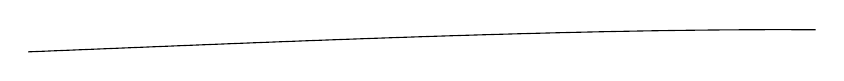
\begin{tikzpicture}\draw (0,0) .. controls (3,.12) and (7,.3) .. (10,.28);\end{tikzpicture}}

f) \deleted{Profondeurs cohomologiques et homotopiques, et ths de Lefschetz locaux et globaux.}

\figure{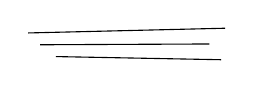
\begin{tikzpicture}\draw (0,.3)--(2.5,.36);\draw (.15,.15)--(2.3,.16);\draw (.35,0)--(2.45,-.04);\end{tikzpicture}}
\margin{165}
\scanpage{167}
Validité des théorèmes de dualité

1) \uline{Dualité globale}
\[
\operatorname{Hom}(F_\bullet,\mathbb{R}^{!}f(G^{\bullet}))\xleftarrow{\sim}\operatorname{Hom}(\mathbb{R}_{!}f(F_\bullet),G^{\bullet})
\]
$f:(X,A_X)\unsure{\text{---}|\longrightarrow}(Y,A_Y)$ morphisme \uline{compactifiable} et \uline{\unsure{lissifiable}} de préschémas, annelés par $A_X$ et $A_Y$, \deleted{\unsure{des}} faisceaux d'anneaux \deleted{de \uline{torsion}} tels que pour tt pt géom. $\bar{y}$ de $Y$, $\exists n_{\bar{y}}\geq1$ \unsure{que} $n_{\bar{y}}A_{Y,\bar{y}}=\deleted{\text{est un anneau}}0$ $n_{\bar{y}}$ premier à $\operatorname{car}k(\bar{y})$.

2) \uline{Dualité locale}
\[
F_\bullet\simeq\unsure{\underline{D}|D}_X\unsure{\underline{D}|D}_X(F_\bullet)\quad\text{isom,}\quad\unsure{\underline{D}|D}_X(F_\bullet)\text{ à ch. constructible,}
\]
$X$ préschéma \deleted{\unsure{loc.}} noeth. \uline{régulier} annelé par $A_X$ faisceau d'anneaux loc. ct à fibres \deleted{\unsure{noethériennes}} \unsure{qui sont} des anneaux de torsion noethériens, premiers aux car. résiduelles

$R_X^{\bullet}$ un \inserted{complexe de} faisceaux de $A_X$-Modules loc. const., et dualisant \inserted{sur les} fibres \deleted{géométriques}
\[
\unsure{\underline{D}|D}_X(F_\bullet)=\unsure{\mathrm{R}|\mathbb{R}}\mathcal{H}om(F_\bullet,\unsure{A_X|R_X})
\]
\[
F_\bullet\in\operatorname{Ob}D^b(X)
\]
\margin{\figure{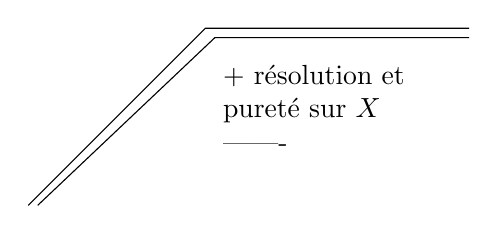
\begin{tikzpicture}[x=1cm,y=1cm]
\draw (0,0)--(2.25,2.25)--(5.6,2.25);
\draw (.12,0)--(2.37,2.13)--(5.6,2.13);
\node[anchor=north west,align=left] at (2.35,1.9) {+ résolution et\\pureté sur $X$\\-------};
\end{tikzpicture}}}
\margin{166}
\scanpage{168}
\margin{167}
\uline{Réédition d'E. V. T., chap. II} \mspage{(10)}
\margin{Tribu n\textsuperscript{o} 53}

au sens espaces topologiques). On construit par récurrence des intervalles $[a_n,b_n]$ \uline{compacts} tels que $[a_1,b_1]\times\ldots\times[a_n,b_n]\subset U\cap\mathbb{R}^n$.

Vider la p. 75 qui ne servait qu'à préparer Krein-Milman. (Attention : vérifier qu'on ne s'en sert pas à la nouvelle édition d'Intégration).

P. 76, vider les l. 1-8.

P. 78, l. 11, remplacer numérique par convexe.

l. 9-10 du bas : $A$ est fermé parce que $f$ est sci !

l. 2 du bas : En divisant$\ldots$

P. 79, l. 6, fonctions affines.

l. 7, supprimer linéaires.

Une dualité ne vérifiera pas $(D_{\mathrm{I}})$ et $(D_{\mathrm{II}})$. Elle pourra être ``séparante en $F$'' ($\Longleftrightarrow\sigma(F,G)$ séparée) ou ``séparante en $G$''. Séparante voudra dire séparante en $F$ et $G$.

Avant la prop. 1, un laïus : $\unsure{F'|F}$ s'identifie à un sous-espace de $G^*$ $\ldots$ ; plus précisément : Proposition 1.

P. 80, vider les l. 7-12 du bas.

l. 6 du bas, souligner infinie.

l. 1 du bas : continues sur $E$.

Dans cet exemple 2, on définira en forme le dual d'un E. V. T. D'où une dualité entre $E$ et $E'$ séparante en $E'$. Si $E$ est localement convexe séparé, cette dualité est séparante en $E$. On ne dira pas ``dual topologique'' mais dual de $E$ ($E$ porte sa structure d'E. V. T.). Les l. 2-6 de la p. 81 se réduiront à : L'espace vectoriel $E'$ est appelé le dual de $E$. Il n'est pas muni lui-même d'une topologie à moins que cela n'ait été expressément mentionné.

Les top. faibles seront non nécessairement séparées. Dans la déf. 1, noter $B$ la forme bilinéaire. Après la déf. 1, dire qu'on la note souvent $\langle x,y\rangle$. Dire que si $G\subset F^*$, la dualité utilisée est la forme canonique de $F\times F^*\mid F\times G$.

Dire que $\sigma(F,G)$ est localement convexe (référence aux topologies initiales).

Proposition : $\sigma(F,G)$ séparée $\Longleftrightarrow$ dualité séparante en $F$.

P. 82, vider les l. 12-14.
\scanpage{170}
Énoncés plausibles (sur préschéma excellent de dim finie).
\diagram{$\unsure{\underline{D}|D}_X\left\{\begin{array}{l}
\unsure{\underline{D}|D}_c(X)^o\simeq\unsure{\underline{D}|D}_c(X)\\
\unsure{\underline{D}|D}_c^-(X)^o\xrightarrow{\sim}\unsure{\underline{D}|D}_c^+(X)\\
\unsure{\underline{D}|D}_c^+(X)^o\simeq\unsure{\underline{D}|D}_c^-(X)\\
\unsure{\underline{D}|D}_c^b(X)\simeq\unsure{\underline{D}|D}_c^b(X)
\end{array}\right.$}

$F_\bullet\in\operatorname{Ob}\unsure{\underline{D}|D}_c^-(X)$, \inserted{$G^{\bullet}=\unsure{\underline{D}|D}_X(F_\bullet)\in\operatorname{Ob}\unsure{\underline{D}|D}_c^+(X)$} je dis que
\[
(1)\qquad F_\bullet\text{ de Tor-dim finie}\Longleftrightarrow G^{\bullet}\text{ de pseudo dim. inj. finie}
\]
\margin{(**)}
\margin{\diagram{\begin{tikzcd}[ampersand replacement=\&,row sep=small]
\begin{gathered}\relax
[\text{i.e. }\inserted{\exists N\text{ tel que }}\text{pour tt }\deleted{\unsure{G_P}}P\deleted{\in\operatorname{Ob}\unsure{\underline{D}|D}_c}\inserted{\text{faisceau}}\\
\text{constructible, }\operatorname{Ext}^i(P,G^{\bullet})=0\\
\text{pour }i>N]
\end{gathered}\arrow[d,leftrightarrow]\\
\text{fibres géom. }G^{\bullet}_{\bar{x}}\text{ est de dim. inj. finie}\\
\text{(pour les }A\text{-Modules)}
\end{tikzcd}}}

\figure{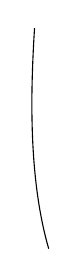
\begin{tikzpicture}[x=1cm,y=1cm]
\draw (0,0)..controls(-.05,-.8) and (-.08,-1.9)..(.18,-2.8);
\end{tikzpicture}}
\uline{N.B.} Si $X$ de dim abs. finie \unsure{on a} pour $G^{\bullet}$ donné ; $G^{\bullet}$ pseudo-dim. inj. finie $\Longleftrightarrow G^{\bullet}$ de dim. injective finie

Dém. de (1). L'implication $\longrightarrow$ formelle, en utilisant que $R_X^{\bullet}$ est de pseudo-dim. injective finie, et
\[
\mathbb{R}\mathcal{H}om^{\bullet}(P_\bullet,\unsure{\underline{D}|D}_X(F_\bullet))
=\mathbb{R}\mathcal{H}om^{\bullet}(P_\bullet,\mathbb{R}\mathcal{H}om^{\bullet}(F_\bullet,R_X^{\bullet}))
\simeq\mathbb{R}\mathcal{H}om^{\bullet}(P_\bullet\overset{\mathbb L}{\otimes}F_\bullet,R_X^{\bullet})
\]
Pour l'implication inverse, utiliser la bidualité pour $F_\bullet\overset{\mathbb L}{\otimes}P$ ----

\uline{NB.} Si les fibres géom $A_{\bar{x}}$ sont Gorenstein, alors en admettant l'équivalence (**), on voit que si $F_\bullet\in\operatorname{Ob}\unsure{\underline{D}|D}_c(X)$ Tor-dim finie $\Longleftrightarrow$ pseudo-dim inj. finie, et $\unsure{\underline{D}|D}_X$ induit une anti-autoequivalence dans la catégorie desdits complexes ...
\margin{169}
\scanpage{171}
\margin{170}
\uline{Réédition des E. V. T., chap. II} \mspage{(7)}
\margin{Tribu n\textsuperscript{o} 63}

l. 7, remplacer $V_\alpha$ par $g_\alpha(V_\alpha)$ ).

P. 55, vider les l. 1-8 du bas.

P. 56, vider les l. 1-2, et 1-12 du bas.

P. 57, l. 1 : II. Limites inductives d'espaces localement convexes. Se donner les $E_\alpha\subset E$ filtrants croissants avec $\bigcup E_\alpha=E$, avec les $E_\beta\longrightarrow E_\alpha$ continues.

Vider les l. 9-14.

l. 13 du bas : Exemple.

P. 58, l. 1, vider 1).

Vider les l. 1-13 du bas.

P. 59, après la déf. 2, donner les voisinages de 0.

(l. 1-8 du bas ; l. 8 du bas, attention au style).

Puis, dire que, pour tout $F$ localement convexe, on a $\mathcal{L}(E,F)=\prod\mathcal{L}(E_i,F)$, et que ceci caractérise la somme directe.

Corollaire : Une limite inductive est quotient d'une somme directe.

Proposition 6. L'injection canonique de $E$ dans $\prod E_i$ est continue. Si $I$ est fini, c'est un isomorphisme d'E. V. T.

P. 60, vider les l. 1-13 du bas.

P. 61, vider les l. 1-5.

Corollaire 1 (ex. 2) : Si les $G_i$ sont fermés, $\sum G_i$ est fermé.

Démonstration : $p_\alpha:E\longrightarrow E_\alpha$ est continu, donc $p_\alpha^{-1}(G_\alpha)$ est fermé, donc $\bigcap p_\alpha^{-1}(G_\alpha)=\sum G_\alpha$ est fermé.

Vider les p. 62, 63, 64 (l. 1-4). On annoncera quelque part qu'une somme directe de complets est complète, mais on le démontrera plus tard à l'aide du th. de Grothendieck.

P. 64, le cor. 1 disparaît, puisqu'il a été glorifié tout de suite après la déf. des sommes directes. Le cor. 2 sera bloqué avec la prop. 7 (dont on conservera les notations), et sera à peu près évident sur la définition catégorique des sommes directes.

Vider la Remarque 2.

P. 65, l. 12, il faut pouvoir dire que $E$ est la limite inductive des $E_n$.

Annoncer : Dans tout le n\textsuperscript{o}, $E$ sera la limite inductive des $E_n$.
\scanpage{172}
\margin{\uline{à vérifier !}}
\margin{\unsure{Généraliser} : aux faisceaux d'anneaux ``\unsure{plus généraux}''.}
\uline{Théorème} Soit $X$ de type \inserted{loc} fini sur le corps $k$, $\dim X\leq n$, $A=\mathbb{Z}/N\mathbb{Z}$, $N$ premier à car. $k$, \deleted{\unsure{Alors}} \inserted{$F$} et $C$ deux $A$-\deleted{\unsure{ét.}}Modules. Supposons que $F$ soit plat $=$ $C$ : fibres injectives ($=$ plates, dans le cas particulier envisagé !). Alors

(i) Si $F$ constructible, alors $\operatorname{Ext}^i(F,\unsure{G|C})=0$ pour $i>2n$.

(ii) Si $k$ est séparablement clos, alors \deleted{\unsure{pour tout}}
\[
\begin{aligned}
\unsure{\mathcal{E}xt^i|\operatorname{Ext}^i}(\deleted{\unsure{A}}\inserted{F},C)&=0&\text{pour }i&>2n\\
\operatorname{Ext}^i(F,C)&=0&\text{pour }i&>2n.
\end{aligned}
\]

\uline{Dém.} (i) se ramène par passage à la limite à (ii). Dans (ii), on peut supposer $k$ sép. clos, et \deleted{un argument général} il suffit de prouver le \uline{premier} alinéa. \inserted{supposer d'abord $C$ : fibres injectives.} Un argument général nous ramène à \deleted{\unsure{le}} vérifier \inserted{la formule} lorsque $F$ est \unsure{quotient} d'un \unsure{produit|générateur} de la forme $i_!(A_{X'})$, où $X'$ affine et $X'\unsure{-|\longrightarrow}X$ étale, \unsure{au} dessus d'un ouvert affine \inserted{$U$} de $X$. Car on se ramène au cas où $X=U$ est aussi affine [car on peut remplacer $X$ par $U$, $C$ par $C|U$]
\margin{\figure{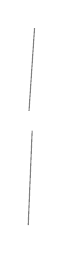
\begin{tikzpicture}[x=1cm,y=1cm]\draw[gray] (0,0)--(0.05,1.2);\draw[gray] (0.01,1.45)--(0.08,2.5);\end{tikzpicture}}}
\margin{171}
\scanpage{173}
\mspage{12}

\uline{Proof}. Follows from [A7, Lemma 3.19 of Section 14].

LEMMA 2. Let $(R,M)$ and $(\bar R,\bar M)$ be two regular local domains of the same dimension $n$ with quotient fields $K$ and $\bar K$ respectively. Assume that $K$ is a subfield of $\bar K$, $\bar R$ has center $M$ in $R$ and $M\bar R=\bar M$. Then $R/M$ can be canonically identified with a subfield of $\bar R/\bar M$; assume that under this identification $\bar R/\bar M=R/M$, i.e., given $x$ in $\bar R$ there exists $y$ in $R$ such that $x-y$ is in $\bar M$. Then given $x$ in $R$ and a positive integer $q$ there exists $y$ in $R$ such that $x-y$ is in $\bar M^q$. Also we have that $K\cap\bar R=R$, $K\cap\bar M=M$, $M^qR=\bar M^q$ for any positive integer $q$, and if $A$ is any ideal in $R$ then $(A\bar R)\cap R=A$ and $A$ is principal if and only if $A\bar R$ is principal, in particular $\bar M^q\cap R=M^q$ for any positive integer $q$. Consequently, any completion of $\bar R$ is also a completion of $R$.

\uline{Proof}. From $M\bar R=\bar M$ we at once have $M^q\bar R=\bar M^q$ for all $q>0$. By induction on $q$ we shall show that given $x$ in $\bar R$ there exists $y$ in $R$ such that if $x-y$ is in $\bar M^q$; for $q=1$ this is given, so assume that $q>1$ and that this is true for $\unsure{q.-1|q-1}$. Then given $x$ in $\bar R$ there exists $z$ in $R$ such that $x-z$ is in $\bar M^{q-1}$; since $\bar M^{q-1}=M^{q-1}R$, $x-z=\sum a_ib_i$ with $a_i$ in $M^{q-1}$ and $b_i$ in $\bar R$, the assumption for $q=1$ tells us that there exists $c_i$ in $R$ and $d_i$ in $\bar M$ such that $b_i=c_i+d_i$, let $y=z+\sum a_ic_i$, then $x-y=\sum a_id_i$ which is in $\bar M^q$.

Now let $x_1,\ldots,x_n$ be a minimal basis of $M$, since $M\bar R=\bar M$
\margin{172}
\scanpage{174}
et $F$ constructible. De plus, par passage à la limite on peut supposer \unsure{les} $C$ également \unsure{constructible}. [Attention, est-il vrai que $C$ est limite ind. \inserted{\uline{\unsure{filtrante}}} des \deleted{\unsure{ses}} faisceaux const. à fibres \uline{injectives} ??].
\margin{?}
\margin{173}
\scanpage{175}
\mspage{11}

and by $f^{-1}(W)$ we shall denote as usual the set theoretic inverse image of the set of points of $W$. It can be immediately verified that if $W$ is irreducible and of co-dimension one so that $Q(W,V)$ is the valuation ring of a real discrete valuation $v$ of $K(V)/k$ then $f^{-1}[W]$ is also irreducible of co-dimension one and it is the center of $v$ on $V^*$.

2. \uline{Auxiliary Lemmas}.

LEMMA 1. Let $(R,M)$ be a regular local domain of dimension $n>1$ with quotient field $K$. Let $x_1,\ldots,x_n$ be a minimal basis of $M$. Let $y_1=x_1$, \deleted{$y_{\unsure{1|i}}=x_{\unsure{1|i}}\mid\alpha_1$} \inserted{$y_i=x_i/x_1$} for $i=2,\ldots,n$ and let $S=R[y_2,\ldots,y_n]$. Then we have $(y_1S)\cap R=M$ so that $R/M$ can be canonically identified with a subfield of $S/(y_1S)$ and then the residues $\bar y_2,\ldots,\bar y_n$ respectively of $y_2,\ldots,y_n$ modulo $y_1S$ are algebraically independent over $R/M$ and hence $S/(y_1S)$ can be identified with the polynomial ring $(R/M)[\bar y_2,\ldots,\bar y_n]$ in $n-1$ variables. Then the canonical homomorphism of $S$ onto $S/(y_1S)$ sets up a one to one correspondence between the maximal ideals in $S$ containing $y_1$ and the maximal ideals in the polynomial ring $S/(y_1S)$, and hence if $P$ is a maximal ideal in $S$ containing $y_1$ and $R_1=S_P\subset K$ and $M_1=PR_1$ then $(R_1,M_1)$ is a regular local domain of dimension $n$ having center $M$ in $R$, $y_1$ is part of a minimal basis of $M_1$ and $R_1/M_1$ is a finite algebraic extension of $R/M$.
\margin{174}
\scanpage{176}
\[
\operatorname{Ext}^p(F,G)
\]
\[
\operatorname{Ext}^{\unsure{p}}(i_!(F),G)\simeq\operatorname{Ext}^p(F,\mathbb{R}i^!(G))
\]
\[
\operatorname{Ext}^*(F,\mathbb{R}i^!(G))\unsure{\Leftarrow|=}E^{pq}=\operatorname{Ext}^p(F,\mathbb{R}^qi^!(\unsure{C|G}))
\]
\margin{\diagram{\begin{tikzcd}[ampersand replacement=\&]Y\arrow[r,hook]\&X\end{tikzcd}}}
\figure{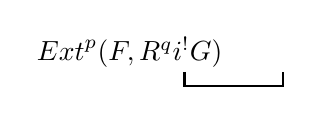
\begin{tikzpicture}[x=1cm,y=1cm]
\node[anchor=west] at (0,0) {$\operatorname{Ext}^p(F,\mathbb{R}^qi^!G)$};
\draw[line width=1pt] (2.0,-0.25)--(2.0,-0.43)--(3.25,-0.43)--(3.25,-0.25);
\end{tikzpicture}}
\[
\operatorname{Ext}^p
\]
\figure{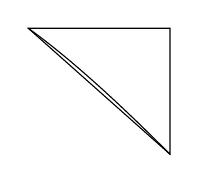
\begin{tikzpicture}[x=1cm,y=1cm]
\draw (0,1.6)--(1.8,1.6)--(1.8,0)--cycle;
\draw (0,1.6) .. controls (0.7,1.1) and (1.5,0.3) .. (1.8,0);
\end{tikzpicture}}
\diagram{$\begin{array}{c@{\quad}c@{\quad}c@{\quad}c@{\quad}c}
\unsure{2d}&\unsure{2d}-1&\unsure{2d}-2&&0\\
\operatorname{Ext}^0,&\operatorname{Ext}^1\ \operatorname{Ext}^2\big/&\operatorname{Ext}^{\unsure{3}}\ \operatorname{Ext}^4\big/&&\big/\operatorname{Ext}^{2d-1},\operatorname{Ext}^{2d}
\end{array}$}
\[
H^p(X,\operatorname{Ext}^q\qquad \deleted{H^{\unsure{n}}}\ H^{\unsure{2d|n}}(X,\operatorname{Ext}^0)+H^{n-1}\operatorname{Ext}^1;
\]
\[
p\leq
\]
\figure{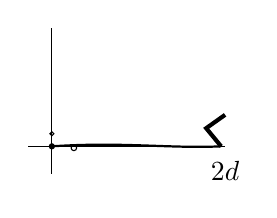
\begin{tikzpicture}[x=1cm,y=1cm]
\draw (-0.3,0)--(2.2,0);\draw (0,-0.35)--(0,1.5);
\fill (0,0) circle(0.04);\draw (0,0.16) circle(0.025);\draw (0.28,-0.02) circle(0.035);
\draw[line width=0.8pt] (0,0)..controls (0.9,0.06) and (1.5,-0.03)..(2.15,0);
\draw[line width=1.5pt] (2.15,0)--(1.96,0.23)--(2.2,0.4);
\node[below] at (2.2,-0.07) {$2d$};
\end{tikzpicture}}
\diagram{$\begin{array}{ccc}
 n\leq2d&n-1\leq2(d-1)&n-3\leq2(d-2)\\
 &\deleted{\unsure{n-1\leq2d-1}}&n-4\leq2(\unsure{2d|d}-2)\\
 &n-2\leq2(d-1)&
\end{array}$}
\[
\deleted{\operatorname{Ext}^*(F,G)\simeq}\qquad\uline{2d-1}
\]
\figure{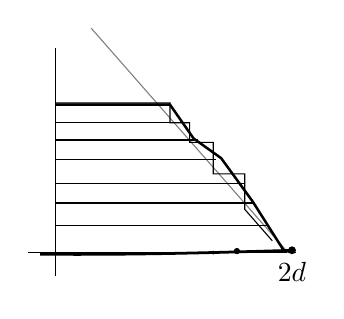
\begin{tikzpicture}[x=1cm,y=1cm]
\draw (-0.35,0)--(3.05,0);\draw (0,-0.3)--(0,2.6);\draw[gray] (0.45,2.85)--(2.95,0);
\draw (0,1.9)--(1.45,1.9)--(1.45,1.65)--(1.7,1.65)--(1.7,1.4)--(2.0,1.4)--(2.0,1.0)--(2.4,1.0)--(2.4,0.55)--(2.75,0.15);
\draw[line width=0.9pt] (0,1.88)--(1.45,1.88)--(1.75,1.45)--(2.1,1.2)--(2.5,0.65)--(2.9,0.02);
\draw (0,1.65)--(1.5,1.65);\draw (0,1.43)--(1.8,1.43);\draw (0,1.18)--(2.04,1.18);\draw (0,0.88)--(2.4,0.88);\draw (0,0.63)--(2.5,0.63);\draw (0,0.35)--(2.7,0.35);
\draw[line width=1pt] (-0.2,-0.02)..controls (1.0,-0.03) and (2.0,0)..(3.02,0.03);
\fill (2.0,0) circle(0.025);\fill (2.3,0.02) circle(0.04);\fill (3.0,0.03) circle(0.05);
\node[below] at (3.0,0) {$2d$};
\end{tikzpicture}}
\[
\mathbb{R}\mathcal{H}om(F,\deleted{\unsure{D}}G)\simeq\mathbb{R}\mathcal{H}om(F\otimes DG,K_X)
\]
\[
\operatorname{Ext}^{\unsure{pq|p+q}}(X;F,\unsure{C|G})\Leftarrow E_2^{pq}=\operatorname{Ext}^{\unsure{pq|p}}(X;\operatorname{Ext}^{-q}(X;G,A_X),A_X)
\]
\[
\operatorname{Ext}^{2d}(X;F,G)
\]
\figure{\begin{tikzpicture}[x=1cm,y=1cm]
\draw (-0.6,1.8)--(2.4,1.8)--(2.4,0)--(0,0);\draw (0,-0.2)--(0,2.2);
\fill (2.4,1.8) circle(0.045);\node[above] at (2.4,1.8) {$2d$};
\end{tikzpicture}}
\figure{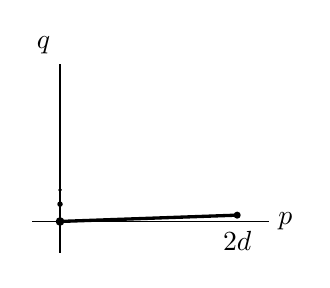
\begin{tikzpicture}[x=1cm,y=1cm]
\draw (-0.35,0)--(2.65,0);\draw (0,-0.4)--(0,2.0);
\draw[line width=1.2pt] (0,0)--(2.25,0.08);\fill (0,0) circle(0.055);\fill (0,0.22) circle(0.035);\fill (0,0.4) circle(0.025);\fill (2.25,0.08) circle(0.045);
\node[above left] at (0,2.0) {$q$};\node[right] at (2.65,0) {$p$};\node[below] at (2.25,0) {$2d$};
\end{tikzpicture}}
\[
\operatorname{Ext}^*(X;F,A_X)\Leftarrow H^p(X,\operatorname{Ext}^q(F,A_X))\qquad 2(d
\]
\[
H^{\unsure{2d|pd}}(X,
\]
\figure{\begin{tikzpicture}[x=1cm,y=1cm]
\draw (0,0)--(3,0);\fill (0,0) ellipse(0.035 and 0.08);\draw (3,-0.04)--(3,0.08);\node[above] at (3,0.08) {$2d$};
\end{tikzpicture}}
\margin{175}
\scanpage{177}
\mspage{67}
\margin{176}

Note that $C_n^{\unsure{v|\nu}}$ is an even function for $n$ even and an odd function for $n$ odd, hence we have
\[
\gamma_n=\begin{cases}
\displaystyle\frac{w_p}{C_n^{1/2\,p}(1)}\,i\pi\int_0^1 C^{1/2\,p}(x)(1-x^2)^{1/2\,p-1/2}\,dx&n\text{ odd}\\[1.5ex]
\displaystyle-\frac{2w_p}{C_n^{1/2\,p}(1)}\int_0^1\log x\ C_n^{1/2\,p}(x)(1-x^2)^{1/2\,p-1/2}\,dx&n\text{ even}
\end{cases}
\]
the result is then proved by evaluating these integrals (see [18a]).

\uline{4.5 Reduction of a singular equation to the Fredholm case}.

We now return to the algebra $\mathcal{G}$ of singular operators on $M$. For each $J\in\mathcal{G}$ and each $x\in M$ we shall define the symbol of $J$ at $x$; this will be a function on $S_x$. Let $\mathbb{H}_xJ$ be the homogeneous part of $J$ at $x$; we define $\mathbb{S}_xJ=\unsure{\mathbf{S}|\mathbb{S}}\unsure{\mathbf{H}|\mathbb{H}}_xJ$, thus $\unsure{\mathbf{S}|\mathbb{S}}_x$ is the composition of the homomorphism $\mathbb{H}_x$ and the isomorphism $\mathbb{S}$.

\uline{Definition 4.5.1.} If $J\in\mathcal{G}$ then the \uline{global symbol} of $J$ is a function on the tangent sphere bundle $S(M)$ defined by
\[
\mathbb{S}_MJ(b)=\unsure{\mathbf{S}|\mathbb{S}}_{\pi(b)}J(b).
\]
Note that $\unsure{\mathbf{S}|\mathbb{S}}_MJ=0$ implies that $\mathbb{H}_xJ=0$ for all $x\in M$ and $J\in\bigcap_{x\in M}\mathcal{F}_x=\mathcal{F}$, so $J$ is completely continuous.
\scanpage{178}
\margin{\figure{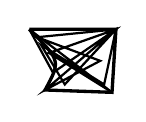
\begin{tikzpicture}[x=1cm,y=1cm]
\draw[line width=1.2pt] (0,0.8)--(1.1,0.8)--(1.05,0)--(0.2,0.03)..controls (0.4,0.4)..(0,0.8);
\draw[line width=0.8pt] (0,0.8)--(1.05,0)--(0.25,0.5)--(1.1,0.8)--(0.2,0.03)--(0.9,0.4)--(0.1,0.7)--(1.1,0.8)--(0.45,0.1)--(0.15,0.6)--(0.95,0.1)--(1.1,0.8)--(0.3,0.25)--(0,0.8);
\end{tikzpicture}}}
\[
\operatorname{Ext}^i(F,G)
\]
\[
\deleted{\unsure{F}}\qquad DG
\]
\[
\begin{aligned}
\mathbb{R}\mathcal{H}om(F,G)&\simeq\mathbb{R}\mathcal{H}om(F,DDG)\\
&\simeq\mathbb{R}\mathcal{H}om(F_{\unsure{\bullet}}\overset{\mathbb L}{\otimes}DG,R_X^{\bullet})
\end{aligned}
\]
\[
F_{\unsure{\bullet|q}}\otimes DG
\]
\figure{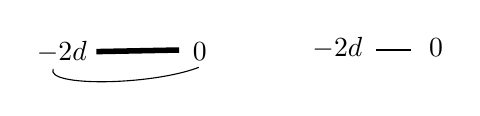
\begin{tikzpicture}[x=1cm,y=1cm]
\node[left] at (0,0) {$-2d$};\node[right] at (1.1,0) {$0$};\draw[line width=2pt] (0,0)--(1.05,0.02);\draw ( -0.55,-0.22)..controls(-0.65,-0.45) and (0.7,-0.43)..(1.3,-0.2);
\node[left] at (3.5,0.05) {$-2d$};\draw (3.55,0.02)--(4.0,0.02);\node[right] at (4.1,0.05) {$0$};
\end{tikzpicture}}
\[
\deleted{\operatorname{Ext}^i}\qquad\mathcal{H}_i(F\otimes DG)\text{ de dim }\leq i
\]
\[
D(F\overset{\mathbb L}{\otimes}DG
\]
\[
\operatorname{Ext}^i(F,G)
\]
\[
\boxed{\operatorname{Ext}^*(F,\unsure{C|G})\Leftarrow E_{\unsure{1|2}}^{pq}=\operatorname{Ext}^{p\deleted{\unsure{+q}}}(F\otimes\operatorname{Ext}^{-q}(G,A_X),A_X)}
\]
\[
\deleted{\unsure{q^4-q\leq q}}\qquad F\otimes\operatorname{Ext}^{2d}(\unsure{C|G},A)
\]
\[
\deleted{\operatorname{Ext}^p(}
\]
\figure{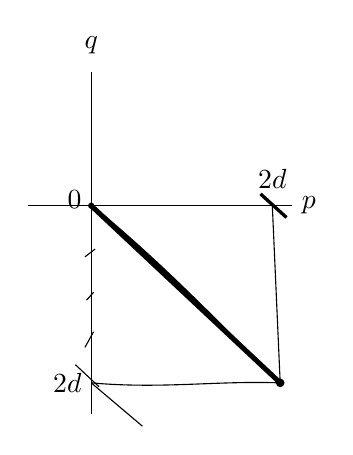
\begin{tikzpicture}[x=1cm,y=1cm]
\draw (-0.8,0)--(2.55,0);\draw (0,1.7)--(0,-2.65);
\node[above] at (0,1.8) {$q$};\node[left] at (0,0.08) {$0$};\node[right] at (2.55,0) {$p$};\node[above] at (2.3,0.1) {$2d$};\node[left] at (0,-2.25) {$2d$};
\draw (0,-2.25)..controls(0.9,-2.33) and (1.6,-2.22)..(2.4,-2.25)--(2.3,0);
\draw[line width=1.8pt] (0,0)--(2.4,-2.25);\draw[line width=0.8pt] (0.03,-0.02)..controls(1.1,-0.9) and (2.0,-1.9)..(2.4,-2.25);
\draw (0,-2.25)--(0.65,-2.8);\draw (-0.2,-2.02)--(0.1,-2.3);
\draw (-0.08,-0.65)--(0.05,-0.55);\draw (-0.06,-1.2)--(0.03,-1.1);\draw (-0.08,-1.8)--(0.03,-1.6);
\fill (0,0) circle(0.04);\fill (2.4,-2.25) circle(0.055);\draw[line width=1.2pt] (2.15,0.15)--(2.48,-0.15);
\end{tikzpicture}}
\margin{$\operatorname{Supp}\operatorname{Ext}^{-q}(\unsure{C|G},A_X)$ de \unsure{codim} $\geq-q$\par
\deleted{de dim $\leq$}\par
donc $\operatorname{Ext}^p(\ ,A_X)$ $=0$ si $p<-q$\par
i.e. $p+q<0$}
\[
\deleted{\operatorname{Ext}^{\unsure{*}}?}\qquad\operatorname{Ext}^{2d}(F,\unsure{C|G})\simeq\operatorname{Ext}^{2d}(F\otimes\mathcal{H}om(\unsure{C|G},A_X),A_X)
\]
\margin{177}
\scanpage{179}
\mspage{68}
\margin{178}

Let $\mathcal{S}_M$ be the algebra of $C^\infty$ functions on $S(M)$; then:

\uline{Theorem 4.5.2.} The map $\unsure{\mathbf{S}|\mathbb{S}}_M:\mathcal{G}\longrightarrow\mathcal{S}_M$ is an epimorphism whose kernel is $\mathcal{F}$, the ideal of completely continuous operators.

Our problem now is to ``regularize'' the equation
\[
(4.5.3)\qquad J\rho=f
\]
that is to reduce it to an equation of Fredholm type. We wish to find an operator $K\in\mathcal{G}$ such that the equation $KJ\rho=Kf$ is of Fredholm type and has the same solutions as the original equation.

Now, if $KJ=Kf$ is of Fredholm type this means that $KJ=I+L$ where $L\in\mathcal{F}$ and then $\mathbb{S}_MKJ=1$. Hence a necessary condition for the existence of a reduction is $\mathbb{S}_MJ(b)\neq0$ for all $b\in S(M)$. This condition is also sufficient:

\uline{Theorem 4.5.4.} If $J\in\mathcal{G}$ then the equation $J\rho=f$ can be regularized if and only if $\unsure{\mathbf{S}|\mathbb{S}}_MJ(u)\neq0$ for all $u\in S(M)$.

\uline{Proof:} We must find an operator $K\in\mathcal{G}$ such that $KL=Kf$ has the same solutions as (4.5.3) and is of Fredholm type. Let $K_1$ be any operator such that $\unsure{\mathbf{S}|\mathbb{S}}_MK_1\cdot\unsure{\mathbf{S}|\mathbb{S}}_MJ=1$; then clearly:
\scanpage{180}
\diagram{\begin{tikzcd}[ampersand replacement=\&,column sep=small,row sep=small]
\ldots\arrow[r]\&\mathbb{R}^i\Gamma_x(F)\arrow[r]\&\unsure{\mathrm{R}|\mathbb{R}}^i\Gamma_X(F)\arrow[r]\&\mathbb{R}^i\Gamma_U(F)\arrow[r]\&\mathbb{R}^{i+1}\Gamma_x(F)\arrow[r]\&\ldots\\
\&\&\times\&\times\&\times\\
\&\mathbb{R}^{-i}\Gamma_X(DF)\&\mathbb{R}^{-i}\Gamma_xDF\arrow[l]\arrow[d]\arrow[dd,bend right=45,no head]\&\mathbb{R}^{-i}\Gamma_U(\unsure{F|DF})\arrow[l]\arrow[d]\arrow[dd,bend left=45,no head]\&\mathbb{R}^{-i-1}\Gamma_XDF\arrow[l]\arrow[d,no head]\arrow[ddl,bend left=20,no head]\&\ldots\arrow[l]\\
\&\&A\&A\&A\\
\&\&\begin{array}{c}\text{dualité parfaite}\\\text{triviale}\\\text{(via \unsure{poncti}\ldots)}\end{array}\&\begin{array}{c}\text{dualité}\\\text{parfaite ??}\end{array}
\end{tikzcd}}
\margin{$f^!\mathbb{R}\mathcal{H}om(F,G)$\par $f^!D=Df^*$}
\margin{$\mathbb{R}\mathcal{H}om(F,G)$\par $D(F\otimes DG)$\par $\mathbb{R}\mathcal{H}om(G,DF)\simeq D(G\overset{\mathbb L}{\otimes}F)$\par $\mathbb{R}\mathcal{H}om(F,D(DG))$\par $\unsure{\mathrm{R}|\mathbb{R}}\mathcal{H}$}
\[
D(H_x^{\unsure{n|i}}(F))\longrightarrow\deleted{\unsure{D\mathcal{H}}}\unsure{\simeq}\mathcal{H}_x^i(DF)_{\unsure{x}}\unsure{\}}
\]
\[
\deleted{\unsure{D}}(F\otimes DG)\simeq D\mathbb{R}\mathcal{H}om(F,\inserted{\unsure{D}}G)
\]
\[
F\longrightarrow DDF
\]
\[
\deleted{H_x^i(F)\longrightarrow}
\]
\figure{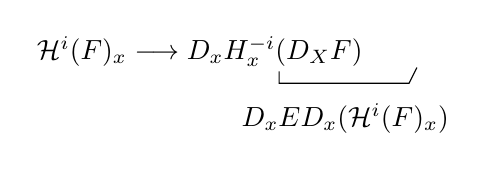
\begin{tikzpicture}[x=1cm,y=1cm]
\node[anchor=west] at (0,0) {$\mathcal{H}^i(F)_x\longrightarrow D_xH_x^{-i}(D_XF)$};
\draw (3.2,-0.25)--(3.2,-0.4)--(4.85,-0.4)--(4.95,-0.2);
\node[anchor=west] at (2.6,-0.85) {$D_x\deleted{\unsure{E}}D_x(\mathcal{H}^i(F)_x)$};
\end{tikzpicture}}
\figure{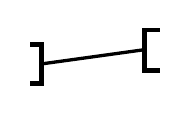
\begin{tikzpicture}[x=1cm,y=1cm]
\draw[line width=1.2pt] (0,0)--(1.3,0.18);\draw[line width=1.7pt] (-0.15,-0.25)--(0,-0.25)--(0,0.25)--(-0.15,0.25);\draw[line width=1.7pt] (1.5,-0.08)--(1.3,-0.08)--(1.3,0.43)--(1.5,0.43);
\end{tikzpicture}}
\margin{$F\otimes DG$\par $-2n,0$}
\figure{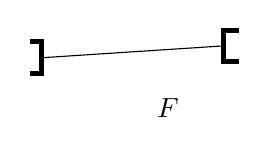
\begin{tikzpicture}[x=1cm,y=1cm]
\draw (0,0)--(2.3,0.15);\draw[line width=1.8pt] (-0.15,-0.2)--(0,-0.2)--(0,0.2)--(-0.15,0.2);\draw[line width=1.8pt] (2.5,-0.05)--(2.3,-0.05)--(2.3,0.35)--(2.5,0.35);
\node[below] at (1.6,-0.4) {$F$};
\end{tikzpicture}}
\figure{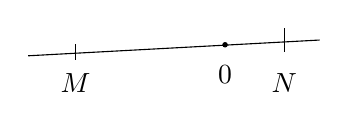
\begin{tikzpicture}[x=1cm,y=1cm]
\draw (-0.4,0)--(3.3,0.2);\draw (0.2,-0.05)--(0.2,0.15);\draw (2.85,0.05)--(2.85,0.35);\fill (2.1,0.14) circle(0.035);
\node[below] at (0.2,-0.1) {$M$};\node[below] at (2.1,0) {$0$};\node[below] at (2.85,-0.1) {$N$};
\end{tikzpicture}}
\figure{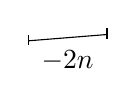
\begin{tikzpicture}[x=1cm,y=1cm]
\draw (0,0)--(1.0,0.08);\draw (0,-0.05)--(0,0.08);\draw (1.0,0.02)--(1.0,0.16);\node[below] at (0.5,0) {$-2n$};
\end{tikzpicture}}
\diagram{\begin{tikzcd}[ampersand replacement=\&,row sep=small]
\text{Tor-dim}_{\unsure{x}}\ F\text{ comprise par }[N,M]\arrow[d,Rightarrow]\\
\text{loc.Inj-dim}^{*}\ D(F)\text{ comprise par }[-2n+N,M]
\end{tikzcd}}
\diagram{\begin{tikzcd}[ampersand replacement=\&,row sep=small]
\text{Inj-dim }F\text{ comprise par }[P,Q]\arrow[d,Rightarrow]\\
\text{Tor-dim }DF\text{ comprise par }[P-2n,Q]
\end{tikzcd}}
\figure{\begin{tikzpicture}[x=1cm,y=1cm]
\node[anchor=west] at (0,0) {$DF\overset{\mathbb L}{\otimes}G\simeq D\mathbb{R}\mathcal{H}om(G,F)$};
\draw (2.95,-0.3)--(2.95,-0.43)--(5.3,-0.43)--(5.4,-0.25);
\node[anchor=west] at (-0.6,-0.8) {$\deleted{DF\otimes DDG\simeq D(F\otimes D\unsure{G})}$};
\node at (4.0,-1.2) {$[P,Q]$};
\draw (2.8,-1.9)--(3.0,-1.9);
\end{tikzpicture}}
\margin{179}
\scanpage{181}
\mspage{24}

LEMMA 11. Let $(R^*,N^*)$ be a quadratic transform of $R$. Then there exists a unique integer $m$ such that $R^*$ is an $m$-th quadratic transform of $R$, also there exists a unique sequence $R=R_{\unsure{o|0}},R_1,\ldots,R_m=R^*$ such that $R_i$ is an immediate quadratic transform of $R_{i-1}$ for $i=1,\ldots,m$. Furthermore $R_{\unsure{o|0}},\ldots,R_m$ are the only quadratic transforms of $R$ which are contained in $R^*$. Also if $v$ is a valuation of $K$ having center $M^*$ in $R^*$ then $R_{\unsure{o|0}},\ldots,R_m$ are the only $q$-th quadratic transforms of $R$ with $q\deleted{\unsure{<}}\inserted{\leq}m$ which are contained in $R_v$ (it is obvious that in each of them $v$ has center at the maximal ideal).

\uline{Proof}. F\deleted{f}ollows from Lemmas 9 and 10 by induction.

DEFINITION 2. \uline{Let} $v$ \uline{be a valuation of} $K$ \uline{having center} $M$ \uline{in} $R$ \uline{and of} $R$-\uline{dimension zero}. \uline{Then} by Lemma 11 above and [A6, Lemma 10] it follows that \uline{for each} $m$ \uline{there exists a unique} $m$-\uline{th quadratic transform} $(R_m,M_m)$ \uline{of} $R$ \uline{such that} $v$ \uline{has center} $M_m$ \uline{in} $R_m$; \uline{and then for all} $m$, $R_m$ \uline{is an immediate quadratic transform of} $R_{m-1}$ \uline{and the} $R_m$-\uline{dimension of} $v$ \uline{is zero}. \uline{We shall say that} $R_m$ \uline{is the} $m$-\uline{th quadratic transform of} $R$ \uline{along} $v$ \uline{and that} $R=R_{\unsure{o|0}},R_1,R_2,\ldots$ \uline{is the quadratic sequence of} $R$ \uline{along} $v$.
\margin{\figure{\begin{tikzpicture}[x=1cm,y=1cm]\draw (0,3.2)..controls(0.4,3.2) and(0.2,2.5)..(0.45,1.9)..controls(0.25,1.4) and(0.35,0.7)..(0.25,0.15)..controls(0.2,0) and(-0.15,0)..(-0.3,0);\end{tikzpicture}}Italicize only the underlined portion}

LEMMA 12. Let $(\bar R,\bar M)$ be an $n$-dimensional regular local domain such that the quotient field $\bar K$ of $\bar R$ contains $K$ as a subfield, $\bar R$ has center $M$ in $R$, $M\bar R=\bar M$ and
\margin{180}
\cotefile{34}
\scanpage{3}
\mspage{1}
\uline{Exposé I}\qquad\deleted{\uline{Action du groupe de monodromie :}}
\uline{Généralités, \inserted{le} th. de monodromie par voie arithmétique.}

0. \uline{Introduction}
\figure{\begin{tikzpicture}[x=1cm,y=1cm]\draw (0,1)..controls(1.2,1.1) and(1.1,0)..(2.2,0)--(12,0.15);\end{tikzpicture}}

0.1. \uline{\unsure{Notations}}. $S=\operatorname{Spec}V$ un trait, $s$ pt fermé, $\eta$ point générique
\[
\mathfrak m=\pi V\inserted{\text{ ``}V\text{''}},\quad k=k(s)\inserted{\text{ ``}V/\mathfrak m\text{''}},\quad K=k(\eta);\qquad p=\text{exp. car. de }k(s).
\]
Le plus souvent, on supposera $V$ hensélien, et \unsure{$S$|même} strictement \unsure{locale|local} i.e. $k$ sép. clos;

\deleted{\unsure{$K$}} $\bar K$ une clôture séparable de $K$, $\bar\eta=\operatorname{Spec}\bar K$;
\[
\pi=\operatorname{Gal}(\bar K/K).
\]
$\ell$ nombre premier. \deleted{Sauf mention du contraire} \deleted{Dans la plus grande partie \unsure{voir}} \inserted{\unsure{Pour toute la première partie du séminaire}, on supposera}
\deleted{L'hyp. de}
\[
\ell\neq\operatorname{car}k
\]

0.2. L'objet du séminaire est l'étude de certaines représentations $\ell$-adiques de $\pi$, provenant de diverses situations géométriques. Une repr. $\ell$-adique de $\pi$ est un \deleted{\unsure{module}} hom. continu
\[
(*)\qquad\pi\longrightarrow\operatorname{Aut}_{\mathbb Z_\ell}(E),
\]
où $E$ est un module de t.f. sur $\mathbb Z_\ell$. On pourra aussi regarder
\[
\pi\longrightarrow\operatorname{Aut}_{\mathbb Q_\ell}(E)
\]
$E$ module de d.f. sur $\mathbb Q_\ell$.

\uline{Exemple} 0.3. $X_K$ schéma algébrique sur $K$, \inserted{$i$ entier.} On suppose que $H^i(X_{\bar K},\mathbb Z/\ell\mathbb Z)$ est un groupe fini, de sorte que
\[
E=H^i(X_{\bar K},\mathbb Z_\ell)\overset{\mathrm{dfn}}=\underset{\nu}{\unsure{\uline{\lim}|\varprojlim}}H^i(X_{\bar K},\mathbb Z/\ell^\nu\mathbb Z)
\]
est un module de t.f. sur $\mathbb Z_\ell$; \deleted{Cette hyp. est} \deleted{\unsure{est}} vérifiée dans les trois cas suivants :

a) On dispose de résolution des sing. \inserted{sous forme de Hironaka (\quad)} des schémas alg. de dim $\leq\dim X$ sur $\bar K$, -- p.ex. $K$ de car. nulle

b) $X$ propre sur $K$.

c) $X$ lisse sur $K$.
\margin{2}
\scanpage{4}
\mspage{2}

\unsure{Comme|Alors} $\pi$ opère sur \deleted{$\unsure{H^iX_{\bar K}}$} $E$ par ``transport de structure'', on trouve une représentation $\ell$-adique $(*)$.

\uline{Exemple} 0.4. Soit $A$ un \deleted{\unsure{schéma en}} groupe algébrique \inserted{comm.} sur $K$.
\deleted{\unsure{comm.}} alors on regarde
\[
 E=T_\ell(A(\bar K))\overset{\mathrm{dfn}}=\varprojlim_\nu {}_{\ell^\nu}A(\bar K)
\]
\deleted{\unsure{Comme}} le groupe ne change pas si on remplace $A$ par $(A^\circ)_{\unsure{\mathrm{red}}}$ (NB. $T_\ell$ est un foncteur exact à gauche nul sur les groupes finis), c'est un \deleted{groupe} \uline{module libre sur} $\mathbb Z_\ell$ de rang égal : $2\alpha+\deleted{\unsure{2}}\mu$, où $\alpha$ ($\mu$) est la dim. de la ``partie'' ``abélienne'' resp. \inserted{``partie''} ``torique'' de $(A_K)^\circ_{\mathrm{red}}$. Ici encore, $\pi$ opère sur $E$ par transport de structure.

\uline{Remarque} 0.5. On peut regarder l'exemple $0.\unsure{3}$ comme étant essentiellement \deleted{un} \inserted{le} cas particulier de l'exemple 0.4, \inserted{pour $i=1$}.
De façon précise, \inserted{on montre que} on a un isom canonique
\[
 H^1(A_{\bar K},\mathbb Z_\ell)\simeq \deleted{\unsure{H^1}}\operatorname{Hom}_{\mathbb Z_\ell}(T_\ell(A(\bar K)),\mathbb Z_\ell),
\]
ou ce qui revient au même, puisque $T_\ell(A_{\bar K})$ est libre de type fini sur $\mathbb Z_\ell$ :
\[
 T_\ell(A(\bar K))=\operatorname{Hom}_{\mathbb Z_\ell}(H^1\unsure{(}A_{\bar K},\mathbb Z_\ell),\mathbb Z_\ell).
\]
D'autre part, \deleted{dans 0.3, si} si \deleted{$i=1$} dans 0.3. $X$ est propre et $i=1$, on trouve
\[
\begin{aligned}
 H^1(X_{\bar K},\mathbb Z_\ell(1))&\simeq\varprojlim_\nu H^1(X_{\bar K},\mu_{\ell^\nu})\simeq T_\ell(\operatorname{Pic}(X_{\bar K}))\\
 &\simeq T_\ell(\underline{\operatorname{Pic}}_{X/K}(\bar K))
\end{aligned}
\]
\margin{3}
\scanpage{5}
\mspage{3}

ou si on préfère
\[
 H^1(X_{\bar K},\mathbb Z_\ell)\simeq T_\ell(\underline{\operatorname{Pic}}_{X/K}(\bar K))\otimes_{\mathbb Z_\ell}\mathbb Z_\ell(-1).
\]

0.6. Lorsque $A$ est un schéma abélien sur $K$, nous verrons que la connaissance du $\pi$-module $T_\ell(A(\bar K))$ donne des informations \unsure{assez} précises sur la structure du \uline{modèle de Néron} de $A$ [\quad], et inversement la \inserted{connaissance du modèle de Néron permet d'obtenir des renseignements complémentaires intéressants sur $T_\ell(A(\bar K))$, et partant sur \unsure{tous les} $H^{\unsure{i|1}}(X_{\bar K})\unsure{?}$ comme $\pi$-modules}.

D'autre part, l'étude des $\pi$-modules plus généraux $H^i(X_{\bar K},\mathbb Z_\ell)$ s'introduit quand on \deleted{\unsure{désire de}} dispose d'un \deleted{modèle} \inserted{schéma} $X$ \deleted{de} sur $S$ de fibre générique $X_K=X_\eta$, et qu'on désire étudier les relations entre \inserted{$H^i(X)$,} $H^i(X_s)$ et $H^i(X_{\bar\eta})$; (p. ex. dans certains cas on pourra montrer $H^i(X_s)\simeq H^i(X_{\bar\eta})^\pi$). Cette \deleted{Deligne, utilisant l'étude} étude locale s'avère comme un outil indispensable pour l'étude \inserted{cohomologique} \uline{globale} d'un morphisme
\[
 f:X\longrightarrow S
\]
avec $S$ régulier de dim 1. \deleted{\unsure{Prenant le}} Dans le cas où $S=\mathbb P^1_k$, et où $f$ ``est'' \deleted{\unsure{disant}} un pinceau \inserted{\unsure{linéaire|linéaires}} de sections hyperplanes d'une variété projective lisse $X_0$ définie sur $k$, on est dans la situation typique de la \uline{théorie de Lefschetz} [\quad]. S'inspirant d'arguments de Lefschetz, Deligne montrera plus tard que si $X_0$ est une surface de degré $\geq4$
\margin{4}
\scanpage{6}
\mspage{4}

dans $\mathbb P^3_k$, alors on a
\[
 \mathbb Z\simeq\operatorname{Pic}(\mathbb P^3)\xrightarrow{\sim}\operatorname{Pic}(X_0),
\]
$k$ étant un corps de car. quelconque.

2. \uline{Rappels sur la structure de} $\pi$.

On suppose $S$ hensélien, i.e. $V$ hensélien.

2.1. Il y a une sous-extension $\widetilde K_{\deleted{\unsure{u}}}$ de $\bar K/K$, qui est la plus grde ss-extension non ramifiée (i.e. étale) \deleted{\unsure{dans}} sur $V$. Si \deleted{$\unsure{\widetilde K_\ell}$ est} $\bar V$ est la clôture normale de $V$ dans $\bar K$, $\widetilde V=\deleted{\unsure{\bar V_\ell}}\bar V\cap\widetilde K_{\deleted{\unsure{u}}}$ la clôture normale dans $\widetilde K_{\deleted{\unsure{u}}}$, alors $\widetilde V_{\deleted{\unsure{u}}}$ est un anneau de valuation discrète tel que
\[
 \deleted{\unsure{\mathfrak m}\widetilde V=\mathfrak m\widetilde V,}
 \qquad \widetilde V\otimes_V k=\bar k
\]
est une \deleted{extension de} clôture séparable de $k$; En d'autres termes, $\widetilde V$ est une \uline{hensélisation stricte} de $V$ p. r. à \deleted{\unsure{une}} la \deleted{\unsure{sa}} clôture séparable $\bar k$ de $k$, et $\widetilde K_{\deleted{\unsure{u}}}$ est le corps des fractions de $\widetilde V$. On pose
\inserted{
\[
\begin{cases}
\widetilde S=\operatorname{Spec}\widetilde V=\text{hensélisé strict de }S\\
\unsure{\bar s}=\operatorname{Spec}\bar k.
\end{cases}
\]
}

\margin{\figure{\begin{tikzpicture}[x=1cm,y=1cm]
\draw (0,0) circle(0.06);\draw (0.06,0)--(0.85,0.02);
\draw (1.02,0.85)..controls(0.9,0.35) and(1.03,0.2)..(1.4,0.08)..controls(1.07,-0.1) and(1.02,-0.35)..(0.94,-0.8);
\end{tikzpicture}}}
\unsure{2.3|2.2}. On se rappelle que \deleted{\unsure{toute}} la donnée de la clôture séparable $\bar K$ de $K$ définit canoniquement une clôture séparable $\bar k$ de $k$.

\deleted{Pour \deleted{\unsure{tout}} \unsure{$n$} \deleted{\unsure{premier à}} \unsure{$p$} \inserted{Si \unsure{$n$} est un} entier \unsure{$n$ premier à} \unsure{$p$} inversible dans $k$, on a
\[
2.1.1.\qquad {}_n\bar k^*\xleftarrow[\unsure{\varphi}]{\sim}{}_n\widetilde V^*\xrightarrow{\sim}\bar K^*
\]
d'où un isomorphisme canonique
\[
\mu_n(\bar K)\simeq\mu_n(\bar k).
\]
Ces isom. sont compatibles avec les \unsure{empilements}
}
\margin{5}
\scanpage{7}
\mspage{5}

schéma fini étale sur $S$, alors on a des isomorphismes
\[
\operatorname{Hom}_S(\bar s,S')\xleftarrow{\sim}\operatorname{Hom}_S(\deleted{\unsure{\bar s}}\widetilde S,S')\xrightarrow{\sim}\operatorname{Hom}_S(\deleted{\unsure{\eta}}\bar\eta,S')
\]
d'où un isom canonique
\[
(2.3.1)\qquad\operatorname{Hom}_S(\bar s,S')\simeq\operatorname{Hom}_S(\bar\eta,S'),
\]
fonctoriel en $S'$ (isom. des \inserted{2} foncteurs ``fibre'' sur la cat. des rev. étales de $S$, définis resp. par les pts géom. $\bar\eta$ et $\bar s$). Faisant $S'=\mu_n$, $n$ \inserted{entier} inversible dans $k$, on trouve en particulier un isom
\[
(2.\unsure{1|3}.2)\qquad \mu_n(\bar s)={}_n\bar k^*\simeq\mu_n(\bar K)={}_n\bar K^*,
\]
d'où par passage à la limite sur les puissances du nb premier $\ell$, $\ell\ne\operatorname{car}.k$ :
\[
(2.3.3)\qquad T_\ell(\bar k^*)\simeq T_\ell(\bar K^*).
\]
\deleted{On notera.} Les deux membres, \deleted{qui} sont des modules libres de rang 1 sur $\mathbb Z_\ell$, \deleted{\unsure{que l'on désigne}} \inserted{qu'on identifie} désormais et désigne par $\mathbb Z_\ell(1)$. \deleted{Sa puissance} \inserted{Sa puiss. tensorielle} nième $(n\in\mathbb Z)$ est notée $\mathbb Z_\ell(n)$. Donc on a
\margin{$(2.3.\unsure{3|4})\qquad\mathbb Z_\ell(1)\simeq\cdots$}
\[
(2.3.4)\qquad \mathbb Z_\ell(n)\simeq\varprojlim_\nu\mu_{\ell^\nu}(\bar k^*)^{\otimes n}\simeq\varprojlim_\nu\mu_{\ell^\nu}(\bar K^*)^{\otimes n}.
\]
Les isomorphismes \deleted{\unsure{sont compatibles aux}} opérations de $\pi$ sur $\mu_{\unsure{n}}(\bar K^*)$ \inserted{et} \unsure{ou} celles de $\pi_0$ sur $\mu_n(\bar k^*)$ etc\ldots compte tenu de l'épimorphisme canonique $\pi\unsure{-|\longrightarrow}\pi_0$.
\margin{6}
\scanpage{8}
\mspage{6}
\margin{\unsure{2}}
\figure{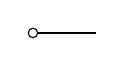
\begin{tikzpicture}[x=1cm,y=1cm]\draw (0,0) circle (.06);\draw (.06,0)--(.8,0);\end{tikzpicture}}

2.2. La sous-extension $\unsure{\bar K_e|\widetilde K_e}$ de $\bar K/K$ est galoisienne, et son groupe de Galois est canoniquement isomorphe au groupe de Galois
\[
(2.2.1)\qquad\pi_0=\operatorname{Gal}(\bar k/k).
\]
On obtient ainsi une suite exacte
\diagram{\begin{tikzcd}[ampersand replacement=\&]
(2.2.2)\quad 1\arrow[r,no head]\&I\arrow[r]\&\pi\arrow[r]\&\pi_0\arrow[r]\&1,
\end{tikzcd}}
où
\[
 I=\operatorname{Gal}(\bar K/\widetilde K)
\]
est ce qu'on appelle le groupe d'\uline{inertie}. \deleted{\unsure{En}} \deleted{\unsure{C'est aussi}} Si on se rappelle que $\widetilde K=$ corps des fractions de $\widetilde V$, \inserted{et que} $\bar K$ est une clôture séparable de $\widetilde K$, on voit donc que $I$ est le groupe de Galois qui correspond à la situation \deleted{\unsure{d'un}} de l'anneau de valuation discrète \uline{strictement local} $\widetilde V$. Si $k$ est sép. clos, on aura $K=\widetilde K$, $V=\widetilde V$, $I=\pi$.

\uline{L'objet du séminaire est} plutôt \uline{l'étude des représentations $\ell$-adiques du groupe d'inertie} $I$. (Ce groupe, ou son image par la représentation $\ell$-adique envisagée, \deleted{\unsure{peut dans le}} est parfois appelé \uline{groupe de monodromie locale}) Il revient au même de dire qu'on s'attachera surtout à étudier les repr. $\ell$-adiques d'un groupe $\pi$, lorsque $k$ est sép. clos. Dans certaines situations cependant, on aura une représentation d'une extension
\margin{7}
\scanpage{9}
\mspage{7}

(2.2.2), et on ne se bornera pas \deleted{\unsure{et}} à étudier sa restriction à $I$. \deleted{\unsure{Pour}} On verra que \deleted{toute} \inserted{parfois} le fait qu'une représentation de $I$ se prolonge à $\pi$ impose à cette représentation des restrictions draconiennes.

2.3.

2.4. Rappelons la structure de $I$. Soit $p$ l'exposant caractéristique de $k$, \deleted{Alors} et soit $P$ \deleted{\unsure{le}} un \deleted{plus grand} sous-groupe de Silow de $I$ ($P=1$ si $p=1$ i.e. $k$ de car. nulle). Alors $P$ \uline{est invariant}, i.e. on a une suite exacte
\diagram{\begin{tikzcd}[ampersand replacement=\&]
(2.4.1)\quad1\arrow[r,no head]\&P\arrow[r]\&I\arrow[r]\&I_t\arrow[r]\&1,
\end{tikzcd}}
où $I_t$ \inserted{(partie ``tame'' du groupe d'inertie $I$)} est un groupe profini premier à $p$, d'autre part on a un isomorphisme canonique
\[
(2.4.2)\qquad I_t\simeq\prod_{\ell\ne p}\mathbb Z_\ell(1)
\]
Le deuxième est obtenu ainsi. Le groupe $P$ est le groupe de Galois \deleted{de}
\[
(2.4.3)\qquad P=\operatorname{Gal}(\bar K/\bar K_t),
\]
où $\bar K_t$ est la plus \deleted{\unsure{grande}} grde sous-extension \uline{modérément ramifiée} de $\bar K/K$ \inserted{(val. : $V$)}, ou encore de $\bar K/\widetilde K$ (val. : $\widetilde V$). Celle-ci s'obtient, \unsure{en termes|en donnant}
\margin{8}
\scanpage{10}
\mspage{\unsure{9|8}}

d'un uniformisant \deleted{$\unsure{\varpi}$} $t$ de $V$, \inserted{donc de $\widetilde V$}, comme la réunion des sous-extensions \deleted{\unsure{abéliennes}} Kummeriennes
\[
(2.4.4)\qquad K_n=\widetilde K(\sqrt[n]{t})\subset\bar K,
\]
où $n$ parcourt les entiers $>0$ premiers à $p$.
Le groupe de Galois de cette extension $K_n$ est naturellement isomorphe au groupe
\[
\mu_n(\bar K)={}_n\bar K^*
\]
des racines nièmes de l'unité dans $\bar K$, et par passage à la limite on trouve
\[
 I_t=\operatorname{Gal}((\varinjlim_n K_n)/K)\simeq\varprojlim_n\operatorname{Gal}(K_n/K,\deleted{\unsure{\bar K}}\unsure{1}),
\]
i.e (2.4.2).

\uline{Remarque} 2.5. On notera que par définition, le sous-groupe $P$ de $I$ est stable par \uline{tout} autom. de $I$, en particulier par les automorphismes induits par les autom. int. de $\pi$. Donc $\pi$ opère par passage au quotient sur $I/P=I_t$; \deleted{On constate aussitôt que} dans cette opération, le \deleted{cette \unsure{opération}} ss-groupe $I$ de $\pi$ opère évidemment trivialement, $I_t$ étant commutatif, on en tire en fait une opération de $\pi/I\simeq\pi_0$ sur $I_t$. \deleted{\unsure{Compte tenu}} On vérifie trivialement que
\margin{9}
\scanpage{11}
\mspage{9}

cette opération, via l'isomorphisme (2.4.2), \deleted{n'est} n'est autre que celle qui provient de \deleted{l'isomorphisme de} \inserted{l'opération naturelle} de $\pi_0$ sur les facteurs $\mathbb Z_\ell(1)$, via l'expression (2.3.3) de $\mathbb Z_\ell(1)$.

Bien entendu, pour tout $\ell$ \unsure{\deleted{\unsure{on a}}\inserted{il existe}|\uline{il existe}} \unsure{des} isomorphismes
\[
\mathbb Z_\ell(1)\simeq\mathbb Z_\ell,
\]
dont le choix revient au choix d'un syst. cohérent de racines \inserted{primitives} $\ell^\nu$-ièmes de 1 dans $\bar K$; Mais on fera attention qu'il n'y a pas de façon naturelle de faire ce choix, et que c'est l'expression intrinsèque (2.4.2) qui seule \deleted{\unsure{peut}} tient compte des opérations naturelles de $\pi_0$ sur le premier membre.
\margin{10}
\scanpage{12}
\mspage{10}

3. \uline{Comportement par \deleted{\unsure{base}} $S$ variable}.

Soit
\[
(3.1)\qquad f:S'=\operatorname{Spec}(V')\longrightarrow S=\operatorname{Spec}V,
\]
un morphisme \uline{dominant} de traits, \deleted{Alors} donc $f(s')=s$, $f(\eta')=\eta$. La donnée d'une \deleted{extension} \inserted{clôture} séparable \deleted{\unsure{nous donne}} $\bar K'$ de $K'$ en définit une $\bar K$ de $K$, à savoir la clôture séparable de $K'$ dans l'extension $\bar K'$. Alors $\widetilde K$ est contenue dans $\widetilde K'$, et $\widetilde V$ dans $\widetilde V'$. L'hom d'inclusion $\widetilde V\unsure{\hookrightarrow|\subset}\widetilde V'$ définit ainsi un hom $\bar k\longrightarrow\bar k'$, correspondant à \deleted{l'hom} \inserted{un} diagramme commutatif de corps.

\diagram{\begin{tikzcd}[ampersand replacement=\&]
(3.2)\quad K'\arrow[r,no head]\arrow[d,no head]\&\widetilde K'\arrow[r,no head]\arrow[d,no head]\&\bar K'\arrow[d,no head]\\
K\arrow[r,no head]\&\widetilde K\arrow[r,no head]\&\bar K
\end{tikzcd}}
\diagram{\begin{tikzcd}[ampersand replacement=\&]
(3.3)\quad V'\arrow[r,no head]\arrow[d,no head]\&\widetilde V'\arrow[d,no head]\\
V\arrow[r,no head]\&\widetilde V
\end{tikzcd}}
\diagram{\begin{tikzcd}[ampersand replacement=\&]
(3.4)\quad k'\arrow[r,no head]\arrow[d,no head]\&\bar k'\arrow[d,no head]\\
k\arrow[r,no head]\&\bar k
\end{tikzcd}}

On trouve ainsi un diagramme commutatif d'extensions, induit par $\operatorname{Gal}(\bar K'/K)=\pi'\longrightarrow\operatorname{Gal}(\bar K/K')=\pi$ :
\diagram{\begin{tikzcd}[ampersand replacement=\&]
1\arrow[r,no head]\&\unsure{I'|P'}\arrow[r,no head]\arrow[d]\&\pi'\arrow[r,no head]\arrow[d,no head]\&\pi'_0\arrow[r,no head]\arrow[d,no head]\&1\\
(3.5)\quad1\arrow[r]\&I\arrow[r,no head]\&\pi\arrow[r]\&\pi_0\arrow[r]\&1
\end{tikzcd}}
L'hom $\pi'_0\unsure{-|\longrightarrow}\pi_0$ n'est autre que l'hom
\diagram{\begin{tikzcd}[ampersand replacement=\&]
(3.6)\quad\operatorname{Gal}(\bar k'/k')\arrow[r,no head]\arrow[d,equal]\&\operatorname{Gal}(\bar k/k)\arrow[d,equal]\\
\pi'_0\&\pi_0
\end{tikzcd}}
déduit de (3.4). L'hom $I'\mathrel{\text{---}}I$ s'insère de \unsure{même} dans un diagramme de suites exactes
\diagram{\begin{tikzcd}[ampersand replacement=\&]
1\arrow[r]\&P'\arrow[r,no head]\arrow[d]\&I'\arrow[r]\arrow[d]\&I'_t\arrow[r,no head]\arrow[d,no head]\&1\\
(3.7)\quad1\arrow[r,no head]\&\unsure{p|P}\arrow[r,no head]\&I\arrow[r,no head]\&I_t\arrow[r,no head]\&1
\end{tikzcd}}
\margin{11}
\scanpage{13}
\mspage{11}

Il convient de déterminer l'hom.
\[
(3.8)\qquad I'_t\simeq\prod_{\ell\ne\unsure{p}}\mathbb Z_\ell(1)\longrightarrow\inserted{I_t\simeq}\prod_{\ell\ne p}\mathbb Z_\ell(1)
\]
où on identifie, grâce à l'inclusion $\bar K\subset\bar K'$, les \deleted{\unsure{deux}} groupes $\mathbb Z_\ell(1)$ définis à l'aide de $\bar K$ ou de $\bar K'$ (savoir $T_\ell(\bar K^*)$ et $T_\ell(\bar K'^*)$).

Pour ceci, on regarde les sous-corps (pour $(n,p)=1$)
\[
(3.9)\qquad\begin{cases}
 K_n=\widetilde K(\unsure{\Theta}_n)\subset\bar K_t&\text{où }\Theta_n^n=t,\\
 K'_n=\widetilde K'(\Theta'_n)\subset\bar K'_t&\text{où }\Theta_n'^n=t'
\end{cases}
\]
et on regarde comment
\[
\operatorname{Gal}(K'_n/\widetilde K')\simeq\mu_n(\widetilde K')\xleftarrow{\sim}\mu_n(\widetilde K)
\]
(groupe des racines nièmes $\varepsilon$ de 1 dans $\widetilde K$) opère sur $K_n$. Si $\varepsilon_{K'}$ désigne l'opération sur $K'_n$ définie par $\varepsilon$, donc
\[
\varepsilon_{K'_n}(\Theta'_n)=\varepsilon\Theta'_n
\]
on trouve, si
\[
(3.\unsure{10})\qquad t=\deleted{\unsure{t}}u't'^e\qquad\uline{(e\in\mathbb N,\ u'\in V^*)}
\]
\inserted{$\unsure{0<e}$}
\margin{d'où $\Longleftarrow\boxed{\begin{array}{c}\deleted{\mathfrak m\widetilde V=\unsure{\mathfrak m'^e}}\\\mathfrak mV=\mathfrak m'^e\end{array}}$}
que
\[
\Theta_n^n=u'(\Theta_n'^e)^n
\]
donc, si on pose
\[
(3.\unsure{11})\qquad\Theta_n=\lambda\Theta_n'^e,\qquad\uline{(\lambda\in K'_n)}
\]
on aura
\[
\deleted{(3.\unsure{12})}\qquad\lambda^n=u',
\]
donc \deleted{\unsure{elle}} $\lambda\in\widetilde V'$ \deleted{\unsure{est}} donc $\varepsilon_{K'}(\lambda)=\lambda$
et on trouve
\[
\varepsilon_{K'_n}(\Theta_n)=\underbrace{\varepsilon_{K'_n}(\lambda)}_{\substack{\Vert\\\lambda}}\varepsilon_{K'_n}(\Theta_n'^e)=\lambda(\varepsilon\Theta'_n)^e=\unsure{\varepsilon}^e\unsure{\Theta_n}
\]
\margin{par (3.10)}
\margin{12}
\scanpage{14}
\mspage{12}

en d'autres termes
\[
 \varepsilon_{K'_n}(\Theta_n)=(\varepsilon^e)_{K_n}(\Theta_n)
\]
et par suite
\[
 \varepsilon_{K'_n}|K_n=(\varepsilon^e)_{K_n}.
\]
Passant à la limite sur $n$, on trouve la

\uline{Proposition} 3.12. Si $\mathfrak mV'=\mathfrak m'^e$, alors l'hom. \inserted{can.} (3.8) provenant de (3.5) s'identifie à la multiplication par $e$.
\figure{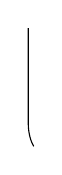
\begin{tikzpicture}[x=1cm,y=1cm]\draw (0,1.5)--(0,.3) .. controls (0,.15) and (.04,.05) .. (.07,0);\end{tikzpicture}}

En particulier, si $e=1$ cet hom. est l'identité, \deleted{\unsure{et}} et à fortiori un isomorphisme. \inserted{Ceci s'applique en particulier si $V'=\widetilde V$.} En fait, on a mieux.

\uline{Prop.} 3.13. Supposons $V'=\widehat V$, \deleted{et $V$ \unsure{excellent}} \inserted{\deleted{et $V$ excellent (i.e. $\widehat K$ sép. sur $K$).}} Alors les hom de suites exactes (3.5) et (3.7) sont des isomorphismes.

\deleted{
$\pi'\longrightarrow\pi$ \deleted{est \unsure{donc}} surjectif, i.e. si $K_1$ est une extension finie séparable de $K$, alors $K_1\otimes_K\widehat K$ est un corps. \deleted{et $I'_t\simeq I_t$} \inserted{La clôture \unsure{normale} $V_1$ de $V$ dans $K_1$ est \uline{\unsure{finie}} \unsure{sur $V$}, par suite $V_1\otimes_V\widehat V=\widehat V_1$ intègre (car $V_1$ est un anneau \inserted{de val. discrète); donc $K_1\otimes_K\widehat K=\widehat V_1\otimes_{\unsure{\widehat V}}\widehat K$ est un corps.}}
(Comme $\pi'_0\longrightarrow\pi_0$ est évidemment un isom., et aussi \inserted{$I'_t\mathrel{\text{---}}I_t$, par \unsure{l'injectivité|l'isomorphisme} de \unsure{$I'_t\mathrel{\text{---}}I_t$}}) on est ramené en fait à examiner $P'\mathrel{\text{---}}P$. Ceci \inserted{[ou directement $\pi'\longrightarrow\pi$, donc $I'\mathrel{\text{---}}I$)} est tjs injectif, d'après les résultats connus de \deleted{approximation} \inserted{continuité} des solutions d'une équation algébrique p. r. aux coefficients, qui \unsure{impliquent|expliquent} que des \unsure{équations|extensions} séparables \uline{voisines} définissent des extensions isomorphes de $\widehat K$. \deleted{D'autre part, c'est surjectif} \inserted{Comme $I'\longrightarrow I$ est surjectif} \inserted{(d'après les résultats} \deleted{\unsure{que donne précisément} l'hypothèse d'excellence}

\uline{Remarque} 3.14. La prop. 3.13. montre que dans la plupart des questions \deleted{\unsure{concernant}} du séminaire, on pourrait supposer $V$ \uline{complet}.
}
\margin{\deleted{\uline{Attention}}}
\margin{$\widetilde V\subset\widetilde{\widehat V}\subset\widehat{\widetilde V}$}
\margin{13}
\scanpage{15}
\mspage{13}

\uline{Dém} a) Comme $\pi'_0\longrightarrow\pi_0$ est évidemment un isom (car $k'/k$ est \unsure{l'ext. triviale}) il suffit de prouver que $I'\simeq I$, et comme $I'_t\xrightarrow{\sim}I_t$ (car $e=1$) il suffit de prouver que $P'\simeq P$.

b) On sait que $\pi'\mathrel{\text{---}}\pi$ est surjectif, i.e pour tte ext. finie sép. $K_1/K$, $K_1\otimes_K\widehat K$ est un \uline{corps} : en effet, la clôture normale $V_1$ de $V$ dans $K_1$ est finie, donc $V_1\otimes_V\widehat V\simeq\widehat V_1$, \deleted{est} \inserted{c'est donc} un anneau de val. discrète ($V_1$ en étant un), donc $K_1\otimes_K\widehat K\simeq\widehat V_1\otimes_V\widehat K$ est un corps.

\deleted{\unsure{D'ailleurs}} \deleted{Quitte à remplacer $V,V'$ par $\widetilde V,\widetilde V'$ et à comparer leurs complétés \unsure{$\widehat{\widetilde V}\simeq\widehat{\widetilde V'}$} de ces deux anneaux, \unsure{on est ramené}}

c) On en conclut, sur les \inserted{hom de} suites exactes, que $I'\mathrel{\text{---}}I$ est surjectif, puis $P'\mathrel{\text{---}}P$ \uline{surjectif}.
Il reste à prouver que $P'\mathrel{\text{---}}P$ est injectif, et pour ceci que $\pi'\mathrel{\text{---}}\pi$ est injectif, \deleted{\unsure{On}} i.e. que toute extension séparable finie $K'_1$ de $K'=\widehat K$ provient d'une ext. sép. finie de $K$. Or ceci résulte du fait connu (``continuité des racines p. r. aux coefficients'') que deux équations séparables \unsure{\deleted{de $K$}|\inserted{de $K$}} à coefficients dans $\widehat K$ \uline{voisins} définissent des \deleted{\unsure{corps}} $\widehat K$-algèbres isomorphes.
\margin{14}
\scanpage{16}
\mspage{14}

3.\unsure{14|15}. Soit $\pi'$ un sous-groupe d'indice fini de $\pi$. Il correspond donc à une extension séparable finie $K'$ de $K$, d'où un normalisé $V'$ de $V$ dans $K'$, qui est un anneau de val. discrète hensélien. Si $k'$ est son corps résiduel, $k'/k$ est une extension finie, donc $\pi'_0\mathrel{\text{---}}\pi'$ \deleted{est} \inserted{induit} un isom de $\pi'_0$ \inserted{$=\operatorname{Gal}(\bar k'/k')$} sur un sous-groupe ouvert de $\pi_0=\operatorname{Gal}(\bar k/k)$. \deleted{D'autre part} \inserted{Il s'impose \unsure{de} vérifier que $\pi'_0\mathrel{\text{---}}\pi'$ est injectif, i.e. que} l'on a \deleted{on voit que}
\[
(3.\unsure{14}.1)\qquad I'=I\cap\pi'
\]
Notons que d'après la théorie générale appliquée à $V'$, on aura pour tt $\ell$ \inserted{nb premier} $\unsure{\ne}p$
\[
(\unsure{3.14.2|2.14.2})\qquad [I'/(I',I')]^{\deleted{\unsure{(\ell)}}(\ell)}\simeq\mathbb Z_\ell(1)
\]
(isom canonique). \deleted{D'autre part,} L'hom $I'_t\mathrel{\text{---}}I_t$ s'identifie, sur $I_t$, à la multiplication par $e$ \inserted{comme dessus}; \deleted{qui} lorsque $k'/k$ est séparable, \deleted{\unsure{p. ex. que}} i.e. l'extension résiduelle de $\widetilde V'/\widetilde V$ \deleted{séparable} \inserted{triviale}, \deleted{\unsure{donc}} p. ex. si $k$ est parfait, alors on peut interpréter $e$ en termes purement ``groupethéorique'' comme
\[
 e=[I:I']=\operatorname{card}I/I'.
\]
\inserted{Sinon, il faut diviser par le facteur inséparable $p^s$ de $k'/k$.}

\deleted{3.\unsure{16}. Il \unsure{reste à examiner}, lorsque \deleted{\unsure{$k'/k$}} \inserted{$I'$} \unsure{est invariant dans} $\pi$ \inserted{dans $I$}, $\unsure{\pi'/K|\pi'/I}$ \unsure{opère sur}}

3.15. Lorsque $\pi'$ est invariant dans $\pi$, \inserted{(i.e. $K'/K$ galoisienne)} il en est de même de \deleted{$\pi'_0$ dans $\pi_0$, puisque (on \unsure{sait} que $k'/k$ est \unsure{purement} galoisienne), donc \unsure{l'hom}} \inserted{$I'=I\cap\pi'$ dans $\pi$ (puisque $I$ est invariant)}, donc \deleted{$\unsure{\pi/\pi'_0}$} \deleted{\unsure{l'hom}} $\pi$ opère sur $I'/(I',I')$ \unsure{,} et par suite sur
\margin{15}
\scanpage{17}
\mspage{15}
\[
(3.\unsure{15}.1)\qquad I'_t=\prod_{\ell\ne p}(I'/(I',I'))(\ell)\simeq\prod_{\ell\ne p}\mathbb Z_\ell(1).
\]
\deleted{Ceci posé, on constate aussitôt que les opérations de $\pi$ \inserted{(Bien entendu, $I'$ opère trivialement \unsure{sur} $I'_{\unsure{ab}}$, donc c'est le groupe $\pi/I'$ qui opère sur $I'_{\unsure{ab}}$ et à fortiori sur $I'_t$.)} Ceci posé, on constate que $I/I'$ opère trivialement sur (3.16.1), et que l'opération de $\pi/I\simeq\pi_0$ sur $I_t$ \unsure{ainsi}}

\deleted{\unsure{Or}} l'isomorphisme \deleted{de $\pi$} (3.16.1) respecte les opérations de $\pi$ sur les deux mbs, où l'opération sur le deuxième mb. \deleted{est} se fait via $\pi_0$ comme expliqué déjà plus haut.

Ceci en fait exprime le fait que l'isom canonique (\unsure{2.15.1|3.15.1}) est compatible aux ``transport de structure''.

En particulier, on trouve que $I\deleted{/I'}$ opère trivialement sur $I'_t$, en d'autres termes

\uline{Corollaire} $3.\unsure{16}$. Pour tt ss-groupe \inserted{ouvert} invariant $I'$ \deleted{d'indice fini} de $I$, l'extension naturelle de $I/I'$ par le quotient $I'_t\simeq\prod_{\ell\ne p}\mathbb Z_\ell(1)$ de $I'$ est une extension \uline{centrale}.
\margin{16}
